\documentclass[12pt]{article}
\usepackage[font=small,labelfont=bf,hypcap=false]{caption}
\usepackage[a4paper,top=20mm,bottom=20mm,right=20mm,left=40mm]{geometry}
\usepackage[utf8]{inputenc}
\usepackage{csquotes}
\usepackage[ngerman]{babel}
\renewcommand{\baselinestretch}{1.5}
\usepackage{blindtext}
\usepackage{tabularx}
\usepackage{ragged2e}
\usepackage{setspace}
\newcommand\hr{\par\vspace{-.5\ht\strutbox}\noindent\hrulefill\par}
\usepackage{longtable}
\usepackage{hyperref}

\usepackage[
natbib=true,
style=numeric,
sorting=none
]{biblatex}
\addbibresource{references.bib}

\usepackage{fancyhdr}
\setlength{\headheight}{14.5pt}
\renewcommand{\headrulewidth}{0pt}
\fancyfoot{}
\fancyhead{}

\usepackage{graphicx}
\graphicspath{{./images}}

\begin{document}
\pagenumbering{gobble}
\begin{titlepage}
    \begin{center}
        % \begin{flushright}
        %     
\includegraphics[width=0.4\textwidth]{universityLogo}\\
        % \end{flushright}
        \vspace{0.5cm}
        \Large{
            \textbf{Hochschule Rhein-Waal}\\
            Fakultät: Kommunikation und Umwelt
        }

        \vspace{3cm}
        \vfill
        \LARGE{
            \textbf{Konzeption und Entwicklung eines Systems zur softwaregestützten Dokumentation von Unternehmensstrukturen für automatisierte Fortschrittsmessung und Werteorientierung 
        }}
        \vfill

        \vspace{1.5cm}
        \LARGE{Bachelorarbeit}
        
        \vfill

        \vspace{1cm}
        \large{vorgelegt von \\}
        \LARGE{Maximilian Oedinger}
    \end{center}
\end{titlepage}
\newpage
\begin{center}
\vspace{20pt}{
    \Large{Hochschule Rhein-Waal}

    \large{Fakultät:  Kommunikation und Umwelt}
}

\vspace{10pt}{
    \large{betreuender Professor:}
    
    \Large{Herr Prof. Dr. Thomas Richter}
}
\vspace{20pt}
\hr
\Large{
    \textbf{Konzeption und Entwicklung eines Systems zur softwaregestützte Dokumentation von Unternehmensstrukturen für automatisierte Fortschrittsmessung und Werteorientierung }
}
\vspace{10pt}

\vspace{5pt}{
    \large{Bachelorarbeit\\im Studiengang\\Medieninformatik\\zur Erlangung des akademischen Grades}
}

\vspace{10pt}{
    \large{\textbf{Bachelor of Science}}
}
\hr
% \vfill
\vspace{10pt}{
    \large{vorgelegt von\\\textbf{Maximilian Oedinger}}
}

\vspace{10pt}{
    \large{En de Bongert 7\\47918 Tönisvorst}
}

\vspace{10pt}{\large{Matrikelnummer:\\25208\\Abgabedatum:\\(Due Date goes here)}}
\end{center}

\fancyhead[C]{\thepage}
\newpage
\pagestyle{fancy}
\pagenumbering{roman}
\begin{abstract}
    Agility plays a big role in managing the complexity of volatile and unpredictable environments, such as project management and project portfolio management, by focussing on the value created for the customer. This leads to the need of systematically scaling agile practices to enterprise level, which can be done by using e.g. the Scaled Agile Framework (SAFe) or Flight Levels and results in big organizational structures with multiple levels of planning and decision making, which have to be documented.
    \newline
    \newline
    For effective decision making in those environments, decisions should be made with metrics in mind that are relevant for the Level in which the decision must be made. This work presents a customizable software solution to document the organizational structure in a way that allows automatic aggregation of such metrics to the level required. These Metrics should be presented in a meaningful manner, providing insights on progress from levels below the one where the decision must be made in and what implications the decision will have on the levels above. Focus of this work is the adaptability of the solution regardless of the framework used to scale agile practices.
    \newline
    \newline
    The solution was evaluated in a case study to determine its usefulness as a webbased software. The results show that the adaptability of the solution is given, but to be useful in a real world scenario, the solution needs to be extended with time-based metrics like velocity, etc. and the ability to not only import data from operational tools like Jira, but also a synchronization of data between the tools, to make the solution usable over time, since the data only represents a snapshot of the current state of the organization.
    \newline
    \newline
    \textbf{Keywords:} agile portfolio management, agile project management, progress tracking, decision making, Flight Levels, Scaled Agile Framework, data aggregation, visualization, web development, mevn stack
\end{abstract}

\newpage
\tableofcontents
\newpage
\addcontentsline{toc}{section}{Abkürzungsverzeichnis}
\section*{Abkürzungsverzeichnis}
\begin{longtable}{p{3cm}p{12cm}}
    Abkürzung & Erklärung \cr
\end{longtable}
\newpage
\addcontentsline{toc}{section}{Symbolverzeichnis}
\section*{Symbolverzeichnis}
\begin{longtable}{p{3cm}p{12cm}}
    Symbol & Erklärung \cr
\end{longtable}
\newpage
\addcontentsline{toc}{section}{Abbildungsverzeichnis}
\listoffigures
\newpage
% dis is probably not da way
% \addcontentsline{toc}{section}{Tabellenverzeichnis}
% \section*{Tabellenverzeichnis}

\newpage
\pagenumbering{arabic}

\section{Einleitung}
\subsection{Motivation}
Kanban ist ein agiles Kommunikations-Framework, welches die Reaktionsfähigkeit und Effizienz eines Projektteams steigern soll. Dies wird durch einen Planungsprozess erreicht, der konstante neue Produktiterationen vorsieht und Arbeitsprozesse von Priorisierung und WIP-Limits abhängig macht.
Klassisch wird Kanban in agilen Softwareentwicklungsprojekten mit Entwicklungsteams von 8 bis 12 Teammitgliedern angewendet.
Die Flight-Level Methode beschränkt das Modell Kanban nicht mehr auf Projektteams, sondern sieht Anwendung in allen Unternehmensebenen, auch Flight-Level genannt, vor. Wird diese Methode erfolgreich auf allen Ebenen eingesetzt, erreicht die Organisation den sogenannten Status der Business-Agilität\cite{agilitaetNeuDenken}. 
Die Methode wurde von Klaus Leopold entwickelt und beinhaltet diese drei Flight-Level, die im Weiteren betrachtet werden\cite{agilesProjektmanagementImBerufsalltag}:

\subsection{Zielsetzung}

\subsection{Methodik}

\subsection{Gliederung der Arbeit}

\newpage
\section{Agile Unternehmensführung}
\subsection{Warum agil}
Agilität im Kontext von Projektmanagement oder auch grundsätzlicher Unternehmensorganisation ist ein alternativer Ansatz für die Planung unternehmensinterner Prozesse, wie z. B. die Umsetzung eines Projekts und steht meist dem sogenannten traditionellen Ansatz gegenüber. Unter diesem traditionellen Ansatz wird für gewöhnlich der lineare Planungsprozess verstanden, welcher voraussetzt, dass Anforderungen vor der Umsetzung klar definiert und dokumentiert sind und somit Risiko minimiert wird. Diese Umstände sind allerdings nicht immer gegeben, bevor ein geplanter Prozess beginnen muss, damit Konkurrenzfähigkeit für ein Unternehmen gegeben ist. Solche zeitkritischen Prozesse sind häufig aber maßgebend für den Erfolg eines Unternehmens, wodurch ein Bedarf für eine Methode entstand, die Anpassbarkeit an sich ändernde Anforderungen und Rahmenbedingungen erlaubt \cite{agilismVsTranditionalApproaches}.

Bei traditioneller Planung erhöht sich durch diese Bedingungen das Risiko die falschen Dinge zum falschen Zeitpunkt zu tun. Agile Methodik erlaubt es diese Prozesse so effektiv wie möglich zu managen, da die Planung nicht linear, sondern iterativ stattfinde. Durch regelmäßige Feedbackschleifen mit Stakeholdern bleibt der Fokus auf Werteorientierung, da sich ändernde Anforderungen regelmäßig in den Planungsprozess der nächsten Iteration einbezogen werden. \emph{Außerdem wird die Projektverantwortung von der Rolle des Projektmanagers ins Team gegeben.} Somit entsteht eine Flexibilität und Anpassbarkeit, welche die hohe Volatilität verringert. Dadurch, dass Dinge erst dann entschieden werden, wenn es notwendig ist, ist allerdings der Gesamtaufwand und die -dauer nicht zu Beginn einschätzbar, sondern immer nur der Aufwand und die Dauer der aktuellen Iteration \cite{agilismVsTranditionalApproaches}.

Ziel bei der Wahl der Planungsmethode ist immer den Erfolg der Umsetzung des geplanten Prozesses zu maximieren. Für Projekte wird dieser Erfolg in zwei Schlüsselfaktoren unterteilt. Kurzfristiger Projekterfolg wird durch die Effizienz definiert, langfristiger Projekterfolg durch Effektivität. Diese beiden Faktoren werden durch Eingrenzung des Projektumfangs, schneller Lieferung, Qualitätssicherung, Kundenzufriedenheit und klare Kommunikation an und zwischen Stakeholdern \cite{traditionalAndAgileOnProjectSuccess}. Im Beispiel des Projektmanagements wurde bereits untersucht, inwiefern die Verwendung von agilen Methoden, den Projekt erfolgt steigert. Dabei stellte sich heraus, dass gerade der Erfolg agiler Projektplanung von der Qualität der Teamarbeit abhängig ist.
Außerdem zeigte sich, dass in den meisten Fällen ein hybrider Ansatz sowohl dem traditionellen als auch dem strikt agilen Ansatz überlegen ist \cite{traditionalAndAgileOnProjectSuccess}.
Hat ein Projekt keinen Bedarf für agile Vorgehensweisen und wird dennoch agil durchgeführt, kann dies zu Verminderung des Projekterfolgs führen.

\subsection{Agile Projektstruktur}
Um die Ziele eines agilen Ansatzes im Projektmanagement zu erreichen, muss die Struktur auch dem agilen Umsetzungsprozess gewachsen sein. Dazu muss das Projekt mit einem iterativen Gedanken geplant werden. Das Projekt muss also nicht nur als ein fertiges Produkt welches am Ende der vollständigen Umsetzung entstanden ist, sondern auch die Zwischenprodukte die am Ende jeder Iteration bereits entstanden sind, betrachtet werden. Das Ziel von agilem PM ist funktionierende Software und das so früh wie möglich, ohne das das vollständige Projekt umgesetzt werden muss. Hierzu verwendet man das Minimum Viable Product(MVP) und Minimum Marketable Features (MMF) \cite{}.  Mit diesen funktionierenden und in sich geschlossenen Iterationen kann während der Umsetzung dann regelmäßig ein Feedbackprozess stattfinden. Diese Feedbackschleifen sind essenziell für die Erhaltung von Werteorientierung und Anpassbarkeit im Verlauf des Projekts \cite{}.

Für MVP und MMF muss das Projekt bis zu einer bestimmten Granularität segmentiert werden. Hierzu verwendet man typischerweise sogenannte Epics und User-Stories. Epics sind in sich geschlossene Bestandteile des Produkts. Mehrere dieser Epics bilden zusammen mit ihrer vollständigen Umsetzung ein MVP oder MMF. Epics können anschließend in User-Stories aufgespalten werden, welche konkrete Funktionalitäten beschreiben. \cite{}

\vspace{20pt}
\begin{center}
    \begin{minipage}{0.8\linewidth}
        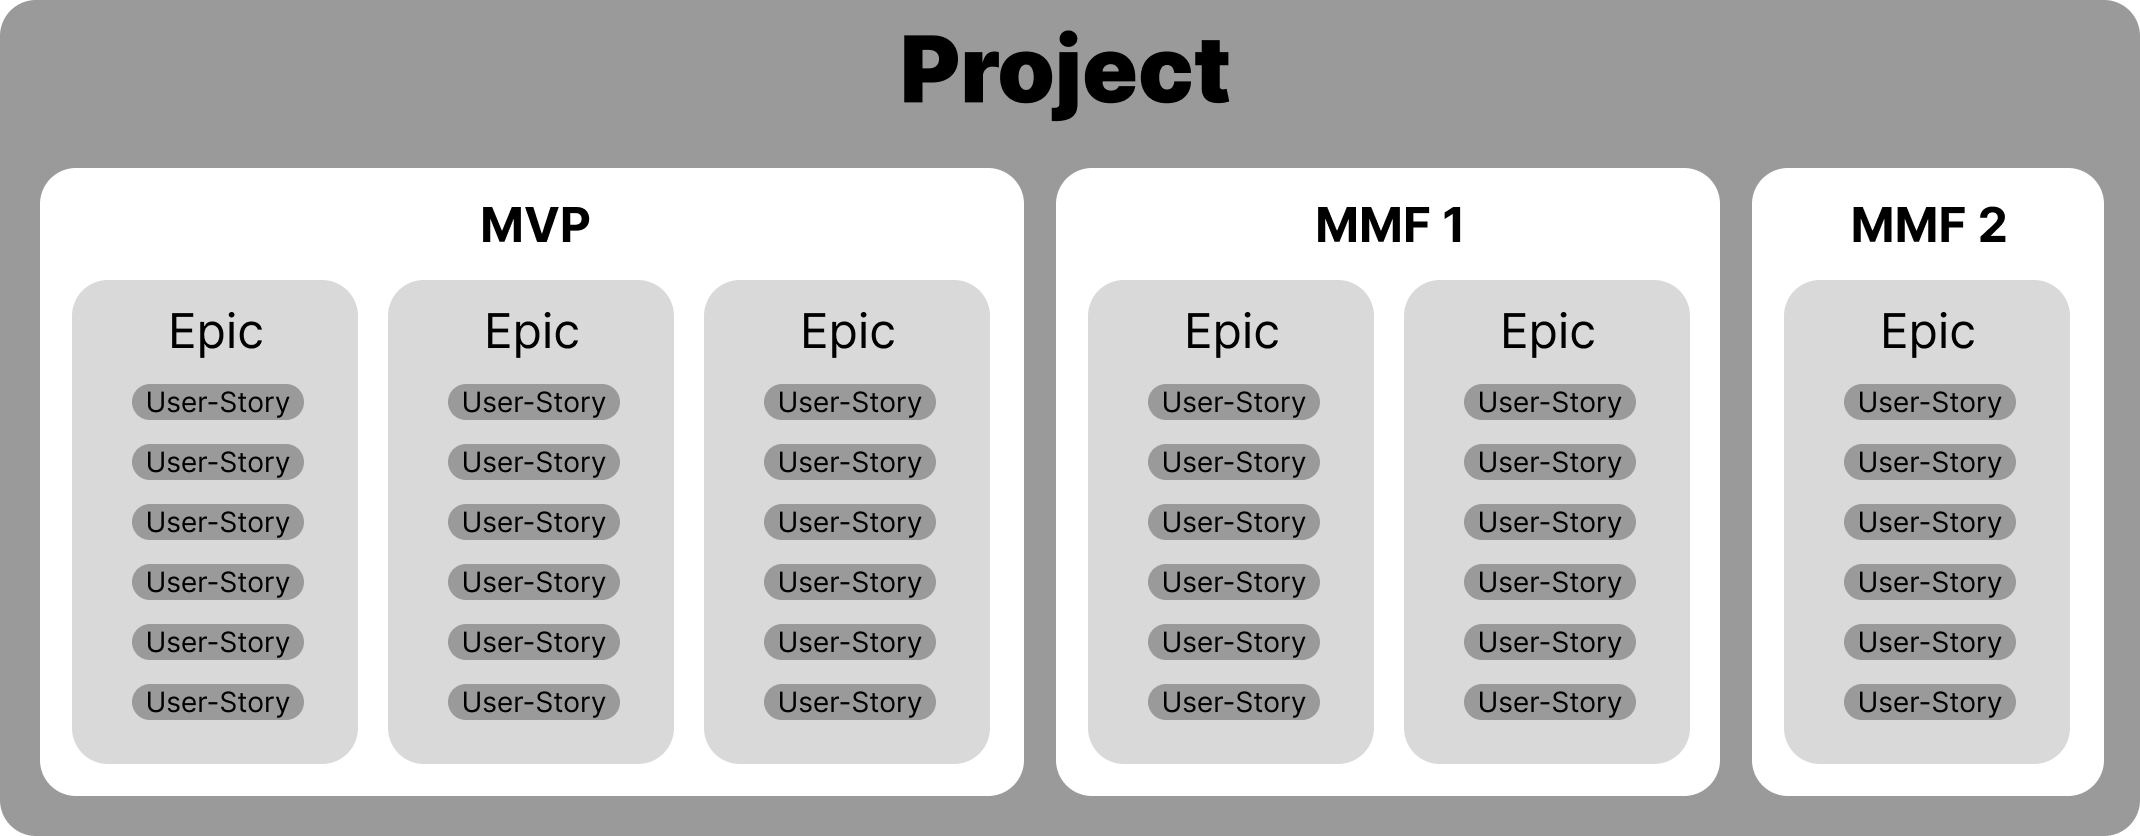
\includegraphics[width=\linewidth]{Project-Tree}
        \captionof{figure}{Agile Projektsegmentierung}
    \end{minipage}
\end{center}
\vspace{20pt}

User-Stories können zum Zeitpunkt der Umsetzung erneut in sogenannte Tasks unterteilt werden. Tasks sind Arbeitspakete die effektiv von einer einzelnen Person an einem Stück bearbeitet werden können. Diese Arbeitspakete sollten von den operativen Projektteammitgliedern definiert werden, da diese die am besten abschätzen können, wie die Beschaffenheit der Tasks sein muss, um Teamressourcen, wie Kapazität und Kompetenzen innerhalb des Teams, optimal zu nutzen. \cite{}

Für die Umsetzung gibt es verschiedene Kommunikations-Frameworks. Die beiden meist vertretenen Frameworks sind Scrum und Kanban. Beide Frameworks bieten Möglichkeiten den iterativen Umsatzprozess mit regelmäßigen Meetings, die ein konkretes Ziel verfolgen, zu strukturieren.

\subsection{Agiles Portfoliomanagement}
Der agile Ansatz kann ebenfalls für das Portfoliomanagement innerhalb eines Unternehmens verwendet werden. Traditionelles Portfoliomanagement oder auch Projekt Portfoliomanagement basiert auf … \cite{}.

Agiles Portfoliomanagement dagegen hat das Ziel Unternehmensziele mit Initiativen oder Projekten zu verknüpfen und somit den Fluss von geleisteter Arbeit auf operativer Ebene zu steuern, um diese Ziele zu erreichen und dabei die Dynamik agiler Frameworks beizubehalten. \cite{}

% In a first cross-case study comparing the application of agile portfolio man- agement in 14 large organisations to existing literature and professional frame- works, Stettina and Hörz [1] point at the characteristics of agile portfolio manage- ment as (1) transparency of resources and work items, improving trust, decision- making, and resource allocation; (2) collaboration, close collaboration based on routinised interaction and artefacts enabling frequent feedback-loops across the domains; (3) commitment to strategically managed portfolios; (4) team orientation, removing unrest in resource allocation and building capabilities in teams.

\subsection{Agile Unternehmensstrukturierung}

\subsection{Beispiel Flight-Level}

\newpage
\section{Analyse}
Im vorherigen Kapitel wurde bereits untersucht wie Projekt- und Projekt-Portfolio-management insbesondere in Kombination mit agiler Methodik die Erreichung strategischer Unternehmensziele unterstützen kann. Durch die regelmäßig anstehenden Entscheidungen besteht der Bedarf für regelmäßiges und vollständiges Reporting, welches für die Entscheidungen herangezogen werden kann, um diese zu objektivieren. In diesem Kapitel soll insbesondere die Automatisierung quantitativer Metriken mit Tools untersucht werden, um Schlüsse für die Umsetzung der Fortschrittsmessung in dieser Arbeit zu ziehen.

\subsection{Reporting für agiles Portfoliomanagement}
Studien zeigten bereits eine positive Korrelation zwischen erfolgreichem Portfoliomanagement und sogenannter Project Portfolio Control (PPC). PPC wird durch drei Faktoren charakterisiert: Projektauswahl, Reporting und Stil der Entscheidungsfindung \cite{ProjectPortfolioControl}.
% Project Portfolio Control and Portfolio Management Performance P.39
% Project Portfolio Control and Portfolio Management Performance P.38
Für die optimale Projektauswahl in PPC wurde bereits untersucht, dass die Entscheidungsfindung optimiert werden kann, indem die Metriken aus dem Reporting, welche für die Entscheidungsfindunge herangezogen werden, mithilfe eines fuzzy Analytic Hierarchy Process (AHP) für eine Priorisierung einzelner Elemente des Portfolios gewichtet werden und anschließen mit der fuzzy TOPSIS Methode in eine Reihenfolge gebracht werden \cite{Mohammed2021}.
% The optimal project selection in portfolio management using fuzzy multi-criteria decision- making methodology P.13
Hieraus lässt sich ableiten, dass es keine generalisierbaren Metriken gibt, die für alle Unternehmen und Projekte gelten, sondern dass die Metriken für jedes Unternehmen und jedes Projekt individuell bestimmt werden müssen. Im Optimalfall sollten also grundsätzlich alle bzw. möglichst viele  Metriken erhoben werden, um sie anschließend zu gewichten.

\subsection{qualitatives vs. quantitatives Reporting}
C. J. Settina und L. Schoemaker \cite{reportingInAgilePortfoliomanagement} untersuchten bereits das Reporting für agiles Portfoliomanagement in einer Fallstudie in mehreren Unternehmen. Aus der Befragung der teilnehmenden Unternehmen ergaben sich folgende Metriken, welche für das Reporting erhoben wurden:

\vspace{20pt}
\begin{center}
  \begin{minipage}{1\linewidth}
    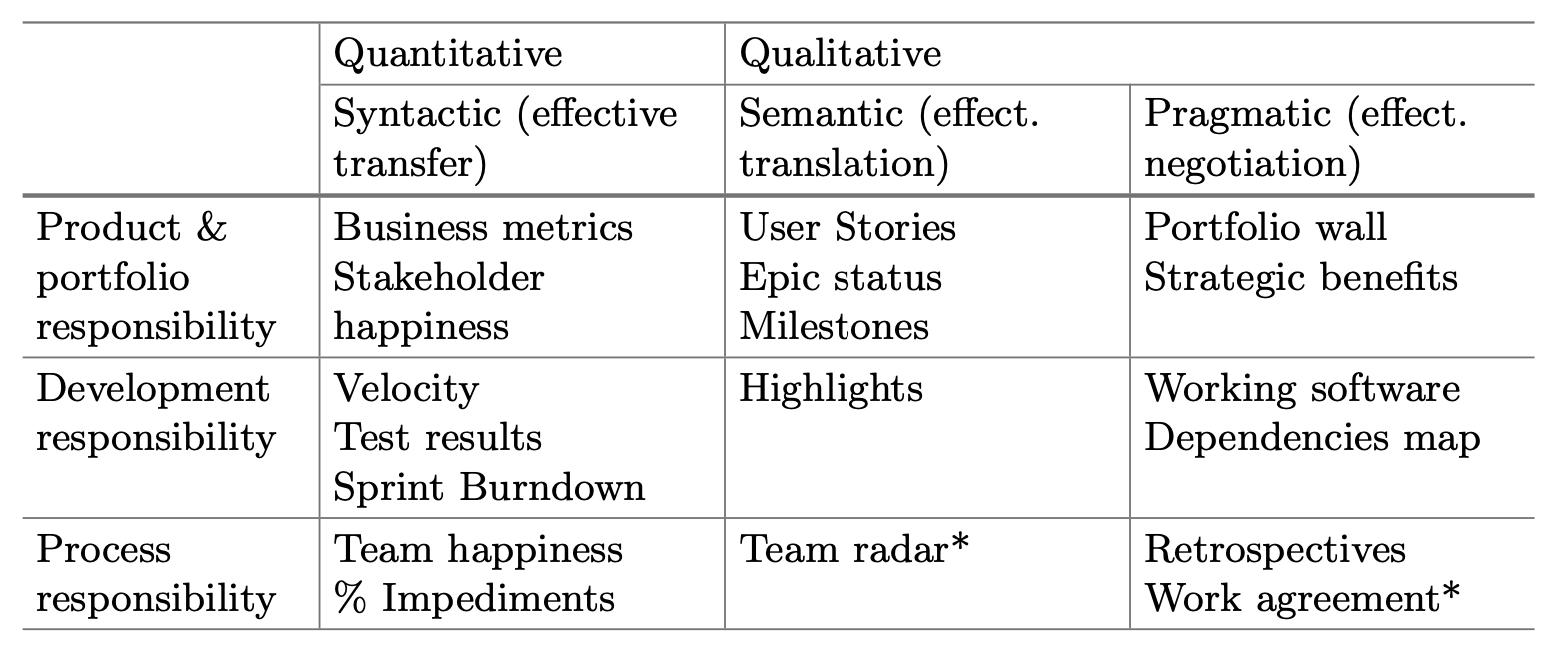
\includegraphics[width=\linewidth]{TableSettinaSchoemaker.png}
    \captionof{figure}{qualitatives und quantitatives Reporting \cite{reportingInAgilePortfoliomanagement} }
  \end{minipage}
\end{center}
\vspace{20pt}


Sie stellten fest, dass für effektives Reporting verschiedene Metriken erhoben werden müssen, welche allgemein in qualitativem und quantitativem Reporting unterteilt werden können.
Qualitatives Reporting zeigt Chancen auf und bietet Kontext, während quantitatives Reporting das Quantifizieren von Elementen und Fortschritt sowie die Validierung von Zielen und geschaffenem Wert ermöglicht.
% Settina und Schoemaker P.212
Aus den gegebenen Metriken kann abgeleitet werden, dass Fortschritt als quantitative Metrik eingeordnet werden kann, da sie vergleichbar mit z. B. Sprint-Burndowns sind, welche letztendlich den Fortschritt über Zeit widerspiegeln.

% \subsection{Reports für Value based Software-Engineering}
% Value-based Software-Engineering(VBSE) ist eine Sammlung von Frameworks für die Entscheidungsfindung in der Softwareentwicklung. VBSE basiert auf der Annahme, dass die Entscheidungen in der Softwareentwicklung auf Basis von einem Kriterium, welches als Wert bezeichnet wird, getroffen werden sollten \cite{}.
% Wert kann hier auf verschiedene Arten definiert werden und kann in mehrere Teile heruntergebrochen werden. Beispiele für Wert sind:
% \begin{itemize}
%   \item Nutzen
%   \item Kosten
%   \item Risiko
%   \item Wert für den Kunden
%   \item Wert für das Unternehmen.
% \end{itemize}

% Unter der Berücksichtigung des Werts können Entscheidungen wertezentiert getroffen werden. Diese Entscheidungen verteilen sich über den gesamten Software-Engineering-Prozess, welcher auch  als VBSE Agenda bezeichnet wird \cite{}.
% Der Prozess kann folgende Teile beinhalten:
% \begin{itemize}
%   \item Requirements Engineering
%   \item Architecting
%   \item Design und Entwicklung
%   \item Verifizierung und Validation
%   \item Planung und Kontrolle
%   \item Risikomanagement
%   \item Qualitätsmanagement
%   \item Mitarbeitermanagement
% \end{itemize}

% \subsection{Teamkoordination}
% Teamkoordination ist ein wichtiger Bestandteil in jeder Form von Projektplanung und -durchführung. In agilen Unternehmen ist Teamkoordination besonders wichtig, da die Teams selbstorganisiert sind und somit die Koordination der Teams untereinander nicht von einer zentralen Instanz übernommen wird und ebenfalls die Projektverantwortung in das Team gegeben wird \cite{}34.
% Somit wird eine gute Teamkoordination kritisch für den Erfolg des Projekts \cite{}.

\subsection{Automatisches Reporting}
Ein weiterer Schluss aus der Arbeit von C. J. Settina und L. Schoemaker \cite{reportingInAgilePortfoliomanagement} ist, dass es sich beim Reporting meist um einen manuellen Prozess handelt, welcher mit wiederkehrendem Aufwand verbunden ist, da die Metriken regelmäßig erhoben werden müssen. Um diesen Prozess des Reportings zu optimieren, sollten qualitative und quantitative Reports unterschiedlich betrachtet werden.

Quantitative Metriken sind quantifizierbar, sodass der Prozess der Erhebung dieser Metriken bei vollständiger Dokumentation aller relevanter Daten automatisierbar ist. Werden diese Metriken dann automatisch erhoben sorgt dies für konsistente, regelmäßige, valide und aktuelle Ergebnissen.

Qualitative Metriken sind dagegen schwer automatisierbar, da sie häufig nicht auf objektiv erfassbaren Daten beruhen. Zur Optimierung kann eine systematische Herangehensweise für die Bestimmung der Metriken definiert werden, um mit deren Hilfe  mehr Konsistenz und Regelmäßigkeit zu gewährleisten. Des Weiteren stellen Sie in ihrer Arbeit die Hypothese auf, dass künstliche Intelligenz in Zukunft eingesetzt werden kann, um auch qualitative Metriken weitestgehend zu automatisieren.
% Settina und Schoemaker P.213

\subsection{Reporting mit digitalen Tools}
Automatisiertes Reporting setzt einen Tool-getriebenen Planungsprozess voraus, um Daten in einem verarbeitbaren Zustand für die Automatisierung zur Verfügung stellen zu können.

\subsubsection{Verwendung von digitalen Tools}
Eine Fallstudie, die mit mehreren IT-Unternehmen durchgeführt wurde, welche aktiv Projekt-Portfoliomanagement betreiben, gibt Empfehlung für eine erfolgreiche Implementierung von Projekt-Portfoliomanagement \cite{guidelinesForPortfoliomanagement}.
Eine dieser Empfehlungen ist die Verwendung eines Systems zur einheitlichen und aktuellen Dokumentation der planungsrelevanten Daten, mit der Reports, die Managemententscheidungen unterstützen, erzeugt werden können.
V. Freitas et al. führten eine weitere Fallstudie durch, die untersuchte wie die Verwendung von webbasierten Tools, speziell dem hier verwendeten ``VALUE''-Tool, Entscheidungsprozesse unterstützen kann \cite{Value-Based-Decision-Making-Case-Study}. Die Ergebnisse zeigten, dass durch die Verwendung des Tools die Entscheidungsfindung und die Qualität der Entscheidungen durch systematische Herangehensweise verbessert wurde.
% V. Freitas, M. Kemppainen, E, Mendes and P. Rodr ́ıguez, “A systematic literature review of value-based decision-making tools,” Submitted to Information and Software Technology.

\subsubsection{Weitere Tools}
Ein vergleichbares Tool zu dem Konzept, welches in dieser Arbeit entwickelt wird, stellt das ebenfalls webbasierte ``Kanbanize'' dar. Es soll ebenfalls Planungselemente in verschiedenen Ebenen miteinander verknüpfen können. Diese Verknüpfungen werden über sogenannte Workflows realisiert, die Abhängigkeiten abbilden können, und dabei sehr spezifisch konfiguriert werden. Dies lässt komplexere Abhängigkeiten als einfache Verknüpfungen zu, erfordert allerdings komplexere Konfigurationen. ``Kanbanize'' stellt sich dabei als All-In-One-Lösung dar und setzt die ausschließliche Verwendung des Tools auch für die operative Arbeit mit Aufgaben voraus, da es keine Synchronisation mit anderen Tools zulässt. Zusätzlich beschränkt sich ``Kanbanize'' auf die Verwendung von Kanban-Boards. Es erlaubt außerdem sehr detaillierte Konfigurationen für das Reporting/Auswerten der aktuell dokumentierten Daten.

\newpage
\section{Konzeption}
Resultierend aus der Analyse soll an dieser Stelle ein Prozess definiert werden, aus denen anschließend ein UX-Konzept und eine prototypische Implementierung entwickelt werden kann.
\subsection{Prozessdefinition / Anforderungsformulierung}
Für Fortschrittsmessung und Werteorientierung müssen Zusammenhänge innerhalb eines Portfolios mit operativen Elementen, deren absoluter Fortschritt tatsächlich gemessen werden kann, dokumentiert werden können. Diese Verknüpfung muss über beliebig viele Ebenen stattfinden können, um möglichst universell und unabhängig von der Unternehmensstruktur verwendbar zu sein.
Operative Elemente, hier genannt Aufgabe, haben einen veränderbaren Status an dem festgestellt werden kann, ob sie fertig sind und somit für den gemessenen Fortschritt einbezogen werden. Aufgaben können außerdem besitzen zudem zwei numerische Werte: Storypoints und Value. Storypoints sollen als relativer Wert die Komplexität der Umsetzung, die mit einer Aufgabe verbunden ist darstellen, während Value den Mehrwert widerspiegelt, welcher durch die Erledigung der Aufgabe entsteht. Die Bezeichnung ist in diesem Fall mit Absicht unspezifisch gewählt, um weitere Komplexität zu vermeiden und den Scope dieser Arbeit zu verkleinern, da zwischen verschiedenen Formen von Mehrwert unterschieden werden kann, wie z. B. Business-, Customer-Value oder auch interner Mehrwert. Ziel dieser Werte ist, die Aufgaben vergleichbarer zu machen, da einige Aufgaben mehr Einfluss auf den Fortschritt haben können als andere. Aufgaben würden somit die Funktion der User-Stories erfüllen.

Die zuvor bereits beschriebene weitere Unterteilung in Tasks spielt für die Fortschrittsmessung oder Werteorientierung und dementsprechend auch für ein Refinement keine Rolle, da Mehrwert und Fortschritt nur entsteht, wenn eine User-Story vollständig umgesetzt wurde und wird deshalb vernachlässigt.

Damit die spezifische Struktur eines Unternehmens abgebildet werden können, muss es möglich sein, verschiedene Ebenen anzulegen, welche die hierarchische Struktur darstellen kann. Innerhalb dieser Ebenen können Elemente angelegt werden, welche mit anderen Elementen in darüber liegenden Ebenen verknüpft werden können.
Die unterste Ebene ist immer die operative Ebene, welche für gewöhnlich als Projekt bezeichnet wird. Optional können Epics verwendet werden, um Aufgaben innerhalb eines Projekts zu gruppieren, sodass mehrere Aufgaben zusammengefasst z. B. ein Feature o. ä. darstellen können.

Der Fortschritt eines Projekts resultiert aus dem Verhältnis von offenen zu erledigten Aufgaben oder Epics, wobei Storypoints und Mehrwert als Faktoren hinzugezogen werden können, um das Verhältnis zu relativieren.

Der Fortschritt eines Planungselements, welches keine Aufgabe oder Projekt ist, wird durch den Gesamtfortschritt der verknüpften Elemente aus der darunterliegenden Ebene aggregiert. Daraus ergibt sich eine Baumartige Struktur, welche die gesamte Planungsstruktur eines Unternehmens abbilden soll.

Um die Evaluierung zu erleichtern und mehrere Szenarien testbar zu machen, können mehrere dieser Strukturen innerhalb der Anwendung existieren, weshalb es eine Ebene gibt, die hier Organisation genannt wird. Organisationen können unabhängig voneinander existieren und eine vollständige Datenstruktur beinhalten.

\subsection{UX-Entwurf für die Abbildung des Prozesses}
Um den Userflow innerhalb des Prototyps darzustellen, wurde ein UX-Entwurf entwickelt, welcher alle Funktionalitäten der Anwendung visuell abbildet und als Grundlage für das Design der Benutzeroberfläche dient. Der Entwurf unterteilt die Anwendung in 7 verschiedene Teile:

\subsubsection{Authentifizierung}
Die Authentifizierung beinhaltet Seiten für den Login und die Registrierung. Außerdem muss der Nutzer sein Passwort zurücksetzen können, indem er einen Reset-Link für seine registrierte E-Mail-Adresse anfordert und über diesen Link ein neues Passwort vergeben kann.

\subsubsection{Menü}
Das Menü besteht aus 2 Seiten. Die Profil-Seite stellt den Nutzernamen und E-Mail-Adresse dar und ermöglicht es dem Nutzer ein JIRA-API-Token für einen JIRA-Import hinterlegen zu können. Auf der Einstellungsseite kann der Nutzer zwischen Light- und Dark-Mode wechseln.

\subsubsection{Organisation}
Auf der Organisationsseite kann der Nutzer alle Organisationen sehen und neue Organisationen erstellen. Beim Erstellen einer Organisation kann der Nutzer sich entscheiden, ob er Epics verwenden möchte. Wenn die Organisation erstellt wird, wird zusätzlich ein Level für Projekte, also die unterste Ebene erstellt. Werden Epics verwendet werden 2 Ebenen standardmäßig erstellt: Project und Epic. Dies hat ebenfalls Auswirkungen auf das Dashboard, da es grundsätzlich alle Levels darstellt. Verwendet eine Organisation allerdings Epics, wird die unterste Ebene, also Epics, nicht mit dargestellt. Außerdem gibt es in den Projekten keine Möglichkeit Epics zu erstellen.

\subsubsection{Dashboard}
Das Dashboard zeigt alle Planungselemente einer Organisation hierarchisch angeordnet an und wie diese miteinander verknüpft sind. Der Nutzer kann je Element anhand einer kleinen Grafik den aktuellen Fortschritt des Elements ablesen. Außerdem hat der User die Möglichkeit den Verlinkungsmodus auszuwählen, wodurch er mit Drag-and-drop neue Verknüpfungen erstellen kann. Durch einen Klick auf das Element gelangt der Nutzer zur Detailansicht des Elements.

\subsubsection{Levels}
Hier kann der Nutzer Ebenen(Levels) erstellen und löschen. Alle Ebenen werden hierarchisch sortiert dargestellt.

\subsubsection{Gruppen}
Je Ebene gibt es eine Gruppenansicht, die alle Elemente(Gruppen) je Level in mit einer kurzen Übersicht über den Fortschritt enthält. Der Nutzer kann neue Gruppen erstellen und auf bestehende Gruppen klicken um zu deren Detailansicht zu gelangen.
In der Gruppendetailansicht gibt es eine detaillierte Übersicht über den Fortschritt des Elements. Der Nutzer kann das Element umbenennen und löschen. Außerdem werden alle verknüpften Elemente aus der darunterliegenden Ebene dargestellt. Mit einem Klick auf eines dieser Elemente kann der Nutzer auch deren Detailansicht aufrufen.

\subsubsection{Projekt}
Die Projektübersicht ähnelt der Gruppenansicht, bietet aber zusätzlich zur einfachen Erstellung neuer Elemente auch die Möglichkeit eines Imports mit einer Excel-Datei. Außerdem kann ein Nutzer, der ein gültiges JIRA-API-Token in seinem Profil gespeichert hat, JIRA-Projekte importieren. Bei einem Import wird nicht nur ein Projekt-Element erstellt, sondern ebenfalls Aufgaben innerhalb des Projekts, die aus der Excel-Datei oder JIRA ausgelesen wurden.
Durch einen klick auf ein Element innerhalb der Übersicht gelangt der Nutzer ebenfalls in eine Detailansicht, welche sich allerdings stark von der einer gewöhnlichen Gruppe unterscheidet.

Der Nutzer kann ein Aufgaben-Board öffnen, in dem er alle Aufgaben des Projekts in drei Spalten sehen kann. Jede Spalte stellt einen der drei Fortschritts-Stati dar: \emph{open}, \emph{in progress} und \emph{done}. Der Nutzer kann mit Drag-and-drop den Status der Aufgaben ändern, indem er sie in die entsprechende Spalte bewegt. Jedes Element besitzt ein Löschsymbol, mit dem das Element, nach einer Bestätigung, gelöscht werden kann. Durch einen Klick auf ein Element öffnet sich ein Pop-up-Pop-up-Fenster mit der Detailansicht der Aufgabe. Diese stellt den Aufgabennamen, die Beschreibung und Storypoints sowie ggf. das zugeordnete Epic dar. Möchte der Nutzer das Epic der Aufgabe wechseln oder sie einem Epic zuordnen, kann er mit einem Drop-down-Menü aus einem der erstellen Epics auswählen. Außerdem kann der Nutzer auch hier die Aufgabe löschen.

Im Aufgaben-Backlog kann der Nutzer alle Aufgaben des Projekts als Listenansicht sehen. Er kann den Aufgabennamen ändern, den Status jeder Aufgabe mit einem Drop-down-Menü anpassen oder die Aufgabe löschen. Außerdem kann der Nutzer hier eine neue Aufgabe erstellen.

Befindet sich das Projekt in einer Organisation die Epics verwendet, gibt es ebenfalls die Epic-Übersicht. Hier werden alle Epics in dem Projekt dargestellt und ihr Fortschritt mit einer Grafik visualisiert. Der Nutzer kann neue Epics erstellen und bestehende Löschen. Klickt er auf ein Epic öffnet sich die Epic-Detailansicht in einem Pop-Pop-up-Fenster, in dem das Epic umbenannt oder gelöscht werden kann. Außerdem wird eine Liste aller Aufgaben ähnlich wie im Backlog angezeigt, die sich in dem Epic befinden. Hier kann der Nutzer zudem Aufgaben, die noch keinem Epic zugeordnet wurden, auswählen und zu diesem Epic hinzufügen. Aufgaben die sich bereits in dem Epic befinden können gelöscht oder nur aus dem Epic entfernt werden. Erstellt der Nutzer an dieser Stelle eine Aufgabe wird diese automatisch dem Epic hinzugefügt.

Das Projekt-Dashboard vereint eine Zusammenfassung des Projekt-Fortschritts mit dem Aufgaben-Board und dem Backlog.

\subsection{Datenaggregation}
Für die Fortschrittsaggregation müssen rekursiv Verknüpfungen zu Elementen der Ebene darunter zusammengefasst werden, bis die Elemente Aufgaben sind, deren Status feststeht. Hierzu beinhalten alle verknüpfbaren Elemente eine Liste mit Referenzen auf verknüpfte Elemente aus der darüber liegenden Ebene. Somit kann überprüft werden welche Elemente der darunterliegenden Ebene mit dem Element, dessen Fortschritt aggregiert werden soll, verknüpft sind. Daraus resultiert eine Liste an Elementen, bei der für jeden Eintrag der Liste genauso wie das für eigentliche Element geprüft werden kann, welche Elemente der darunter liegenden Ebene eine Referenz auf das Element haben. Dies wird so oft wiederholt, bis die verknüpften Elemente Aufgaben sind.

\vspace{20pt}
\begin{center}
    \begin{minipage}{0.8\linewidth}
        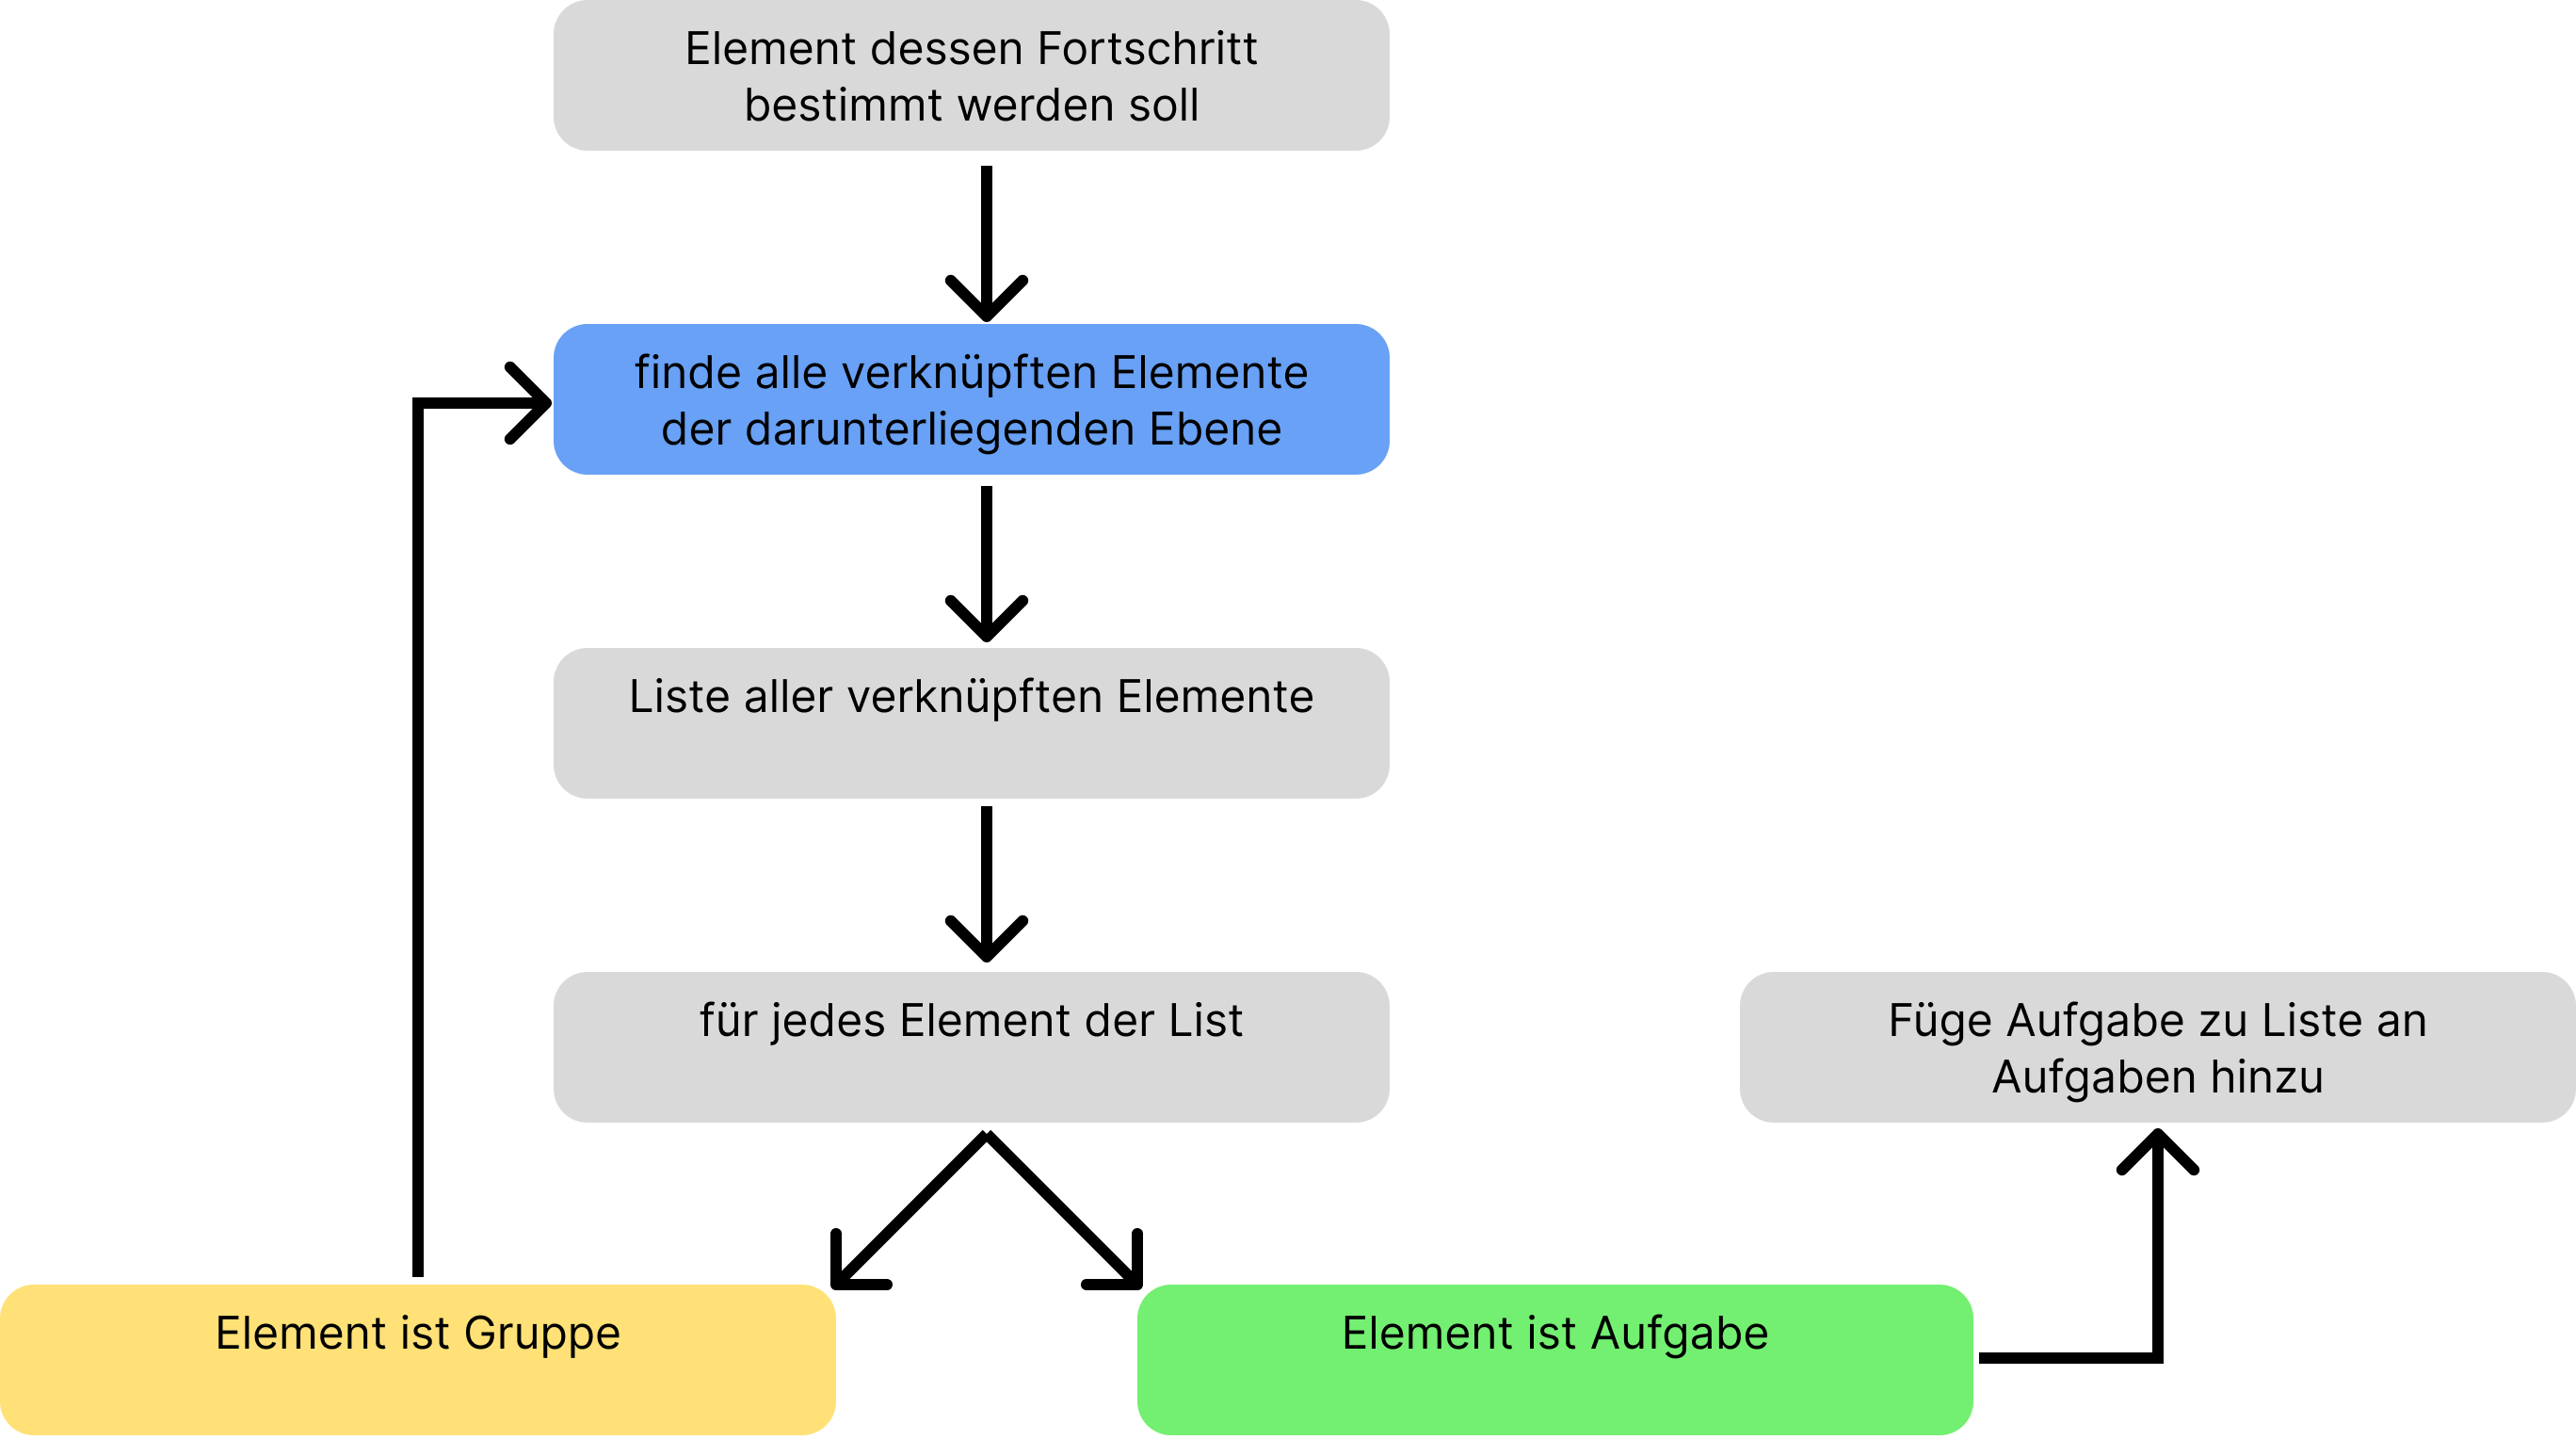
\includegraphics[width=\linewidth]{Fortschrittsaggregation}
        \captionof{figure}{Prozess für Fortschrittsaggregation}
    \end{minipage}
\end{center}
\vspace{20pt}

Die Liste an Aufgaben, die sich am Ende des Prozesses ergibt, kann anschließend nach Aufgaben in den verschiedenen Stati sortiert werden, und entweder die Anzahl an fertigen Aufgaben durch die Gesamtmenge an Aufgaben geteilt, um denn generellen relativen Fortschritt zu bestimmen, oder die Summe der Storypoints aller fertigen Aufgaben durch die Gesamtmenge an Storypoints aller Aufgaben geteilt werden, um den absoluten Fortschritt zu bestimmen.

\newpage
\section{Implementierung}
\subsection{Datenstruktur}
Die Datenstruktur der Anwendung besteht grundsätzlich aus drei abstrakten und fünf konkreten Klassen. Die abstrakten Klassen sind Entitäten, organisationsbasierende Entitäten und verlinkbare Entitäten. Die absoluten Klassen sind Nutzer, Organisation, Level, Gruppe und Aufgabe.

\vspace{20pt}
\begin{center}
    \begin{minipage}{1\linewidth}
        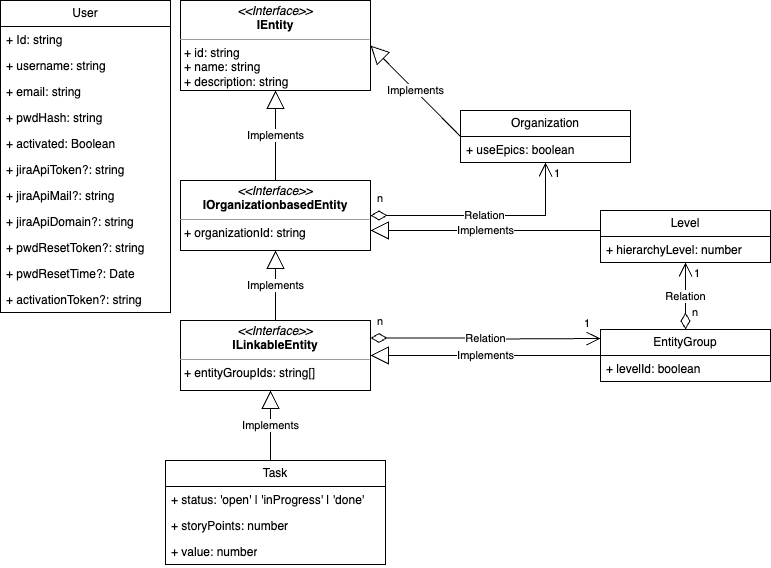
\includegraphics[width=\linewidth]{classDiagramm}
        \captionof{figure}{UML-Diagramm der Datenstruktur}
    \end{minipage}
\end{center}
\vspace{20pt}

Jede absolute Klasse, außer die Nutzer, erben von einer oder mehreren abstrakten Klassen. Entitäten sind allgemeine Objekte innerhalb der Anwendung und stellen die Grundlage der in der Datenbank gespeicherten Datenobjekte dar. Alle Klassen außer Nutzer sind solche Entitäten und implementieren das Interface \verb|IEntity|, welches eine ID zur eindeutigen Identifikation und einen Namen für die Darstellung für den Nutzer beinhaltet. Organisationen und Levels sind direkte Erben dieser Klasse. Die nächste Abstraktionsstufe sind die organisationsbasierenden Entitäten. Diese implementieren zu dem \verb|IEntity| Interface noch \verb|IOrganizationBasedEntity|, welches die ID einer Organisation voraussetzt und die Entität direkt von einer Organisation abhängig macht. Die letzte Abstraktionsstufe sind die verlinkbaren Entitäten. Diese implementieren zu dem \verb|IOrganizationBasedEntity| Interface noch \verb|ILinkableEntity|, welches eine Liste von IDs voraussetzt, mit dem gespeichert wird, mit welchen anderen verlinkbaren Entitäten das Objekt verlinkt ist. Aufgaben und Gruppen sind solche verlinkbare Entitäten.

\subsection{Backend-Architektur}
Das Backend ist eine REST-API, geschrieben mit Node.js und Express in TypeScript und verwendet mongoose als Datenbank-API für MongoDB. Die Architektur beschreibt den Datenfluss mit drei allgemeinen Komponenten: Router, Controller und Service.
Der Router bestimmt für einen Request welche Funktion eines Controllers aufgerufen wird. Die aufgerufene Controller-Funktion beinhaltet die Business-Logik, die an den Request gebunden ist und führt diese aus. Um Daten aus der Datenbank zu holen oder die geholten Daten zu modifizieren gibt es für jede Datenklasse einen Service, der die benötigten Datenbankoperationen implementiert und somit von der Business-Logik trennt. Für die Interaktion mit der Datenbank muss außerdem ein sogenanntes Model definiert werden, welches die Beschreibung der Klasse also der Type in TypeScript mit der Datenbank-Collection und den Objekten darin verknüpft.

\vspace{20pt}
\begin{center}
    \begin{minipage}{1\linewidth}
        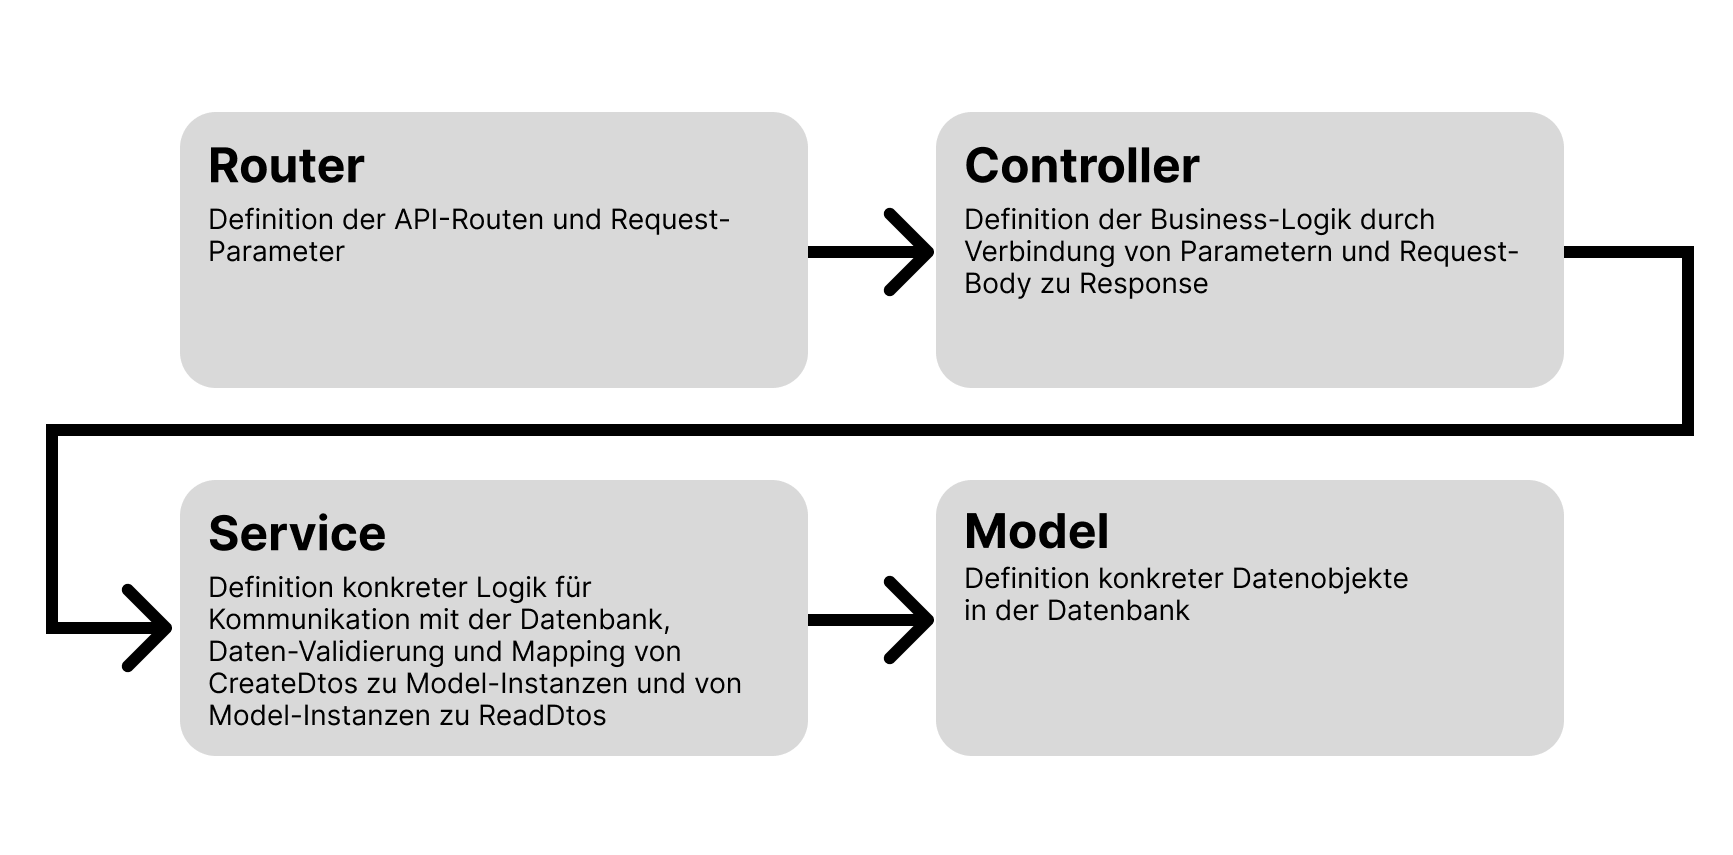
\includegraphics[width=\linewidth]{BE-Struktur}
        \captionof{figure}{Backend Architektur}
    \end{minipage}
\end{center}
\vspace{20pt}

Für die konkrete Kommunikation mit der REST-API werden zu den konkreten Datenobjekten innerhalb der Datenbank zwei weitere Klassen je Objekt-Klasse definiert. Diese Klassen sind sogenannte Data transfer Objects (DTO). DTOs dienen dazu die Kommunikation zu generalisieren und definieren die Daten, die der Konsument der API durch einen Request erhalten kann und die Daten, die ein Konsument der API zur Verfügung stellen kann, um z. B. ein neues Objekt in der Datenbank zu erstellen. Die zusätzlichen Klassendefinitionen werden durch diese zwei Anwendungsfälle in Read- und Create-/Update-DTOs unterteilt. Wie Create-/Update-DTOs zu einem internen Model gemappt werden und wie aus einem internen Model ein Read-Dto gemappt wird, definiert ebenfalls der zum Model zugehörige Service.

Der Aufbau des Backends gleicht dem Aufbau der Klassen-Abstraktion. Es gibt für jede abstrakte Klasse eine Struktur welche jeweils eine abstrakte Implementierung für Router, Controller, Services und Model beinhalten.
Zudem gibt es fünf absolute Strukturen für jede der fünf absoluten Klassen, welche von den verschiedenen abstrakten Strukturen erben.


\vspace{20pt}
\begin{center}
    \begin{minipage}{1\linewidth}
        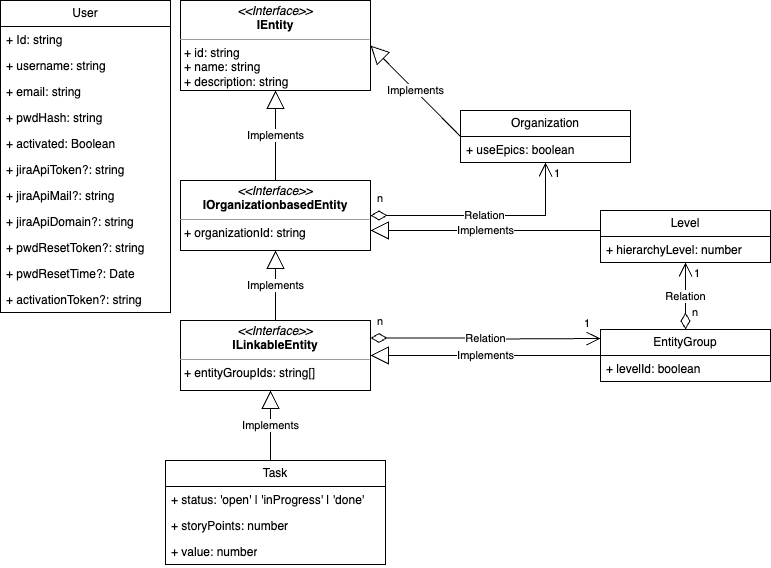
\includegraphics[width=\linewidth]{classDiagramm}
        \captionof{figure}{Abbildung der BE-Struktur}
    \end{minipage}
\end{center}
\vspace{20pt}

hier noch eine detaillierte Beschreibung der Strukturen ????

Eine vollständige Dokumentation der API im Swagger-Format ist unter \url{https://116.203.140.167.nip.io/api-docs/} verfügbar. Dort sind die für den Client zugänglichen Routen inklusive der benötigten Parameter und den zurückgegebenen Daten dokumentiert.

\subsection{Benutzeroberfläche}
Zur initialen Planung wurde zunächst der UX-Entwurf verwendet um die grobe Struktur der Benutzeroberfläche zu entwickeln. Durch die spezifische Entwicklung verschiedener Features sind immer wieder Lücken im Entwurf aufgefallen und wurden duch weitere UI-Elemente erweitert um Funktionalitäten abzudecken, die zuvor nicht innerhalb des Prototypen bedacht wurden. Bis zum fertigen Prototypen haben sich viele der konkreten UI-Elemente verändert, allerdings blieb die Seitenstruktur also welche Informationen auf welches Seite dargestellt wurden identisch.

Für die Implementierung wurde als Frontend-/UI-Framework Vue.js verwendet. Vue.js ist eine Framwork für die Entwicklung von Single-Page-Webanwendungen. Es ist ein JavaScript-Framework, welches auf dem Model-View-ViewModel (MVVM) basiert. Die UI wurde also in verschiedene Komponenten zerteilt. Die Komponenten werden in zwei Kategorien unterteilt: Views und Components. Views sind logisch voneinander getrennte Seiten der Anwendung, während Components kleinere Bestandteile der Views zur vereinfachung der in der View benötigten Logik oder wiederverwendbare UI-Elemente sind. Zur weiteren Strukturierung werden hier noch sogenannte Layouts verwendet. Layouts stellen die Grundstruktur der Anwendung dar, welche von mehreren Views verwendet wird.

Die Anwendung teilt sich zunächst in zwei solcher Layouts: Authentifizierung und eigentliche Anwendung.

Das Layout der Authentifizierung beschreibt nur die Positionierung der relevanten Elemente in der Mitte des Bildschirms, da sich alle Seiten der Authentifizierung diese Eigenschaft teilen.
Das Layout der eigentlichen Seite teilt die Seite in drei Teile, den Header, den Inhalt und einen Footer. Der Header beinhaltet die Navigationsleiste, die den Nutzer durch die Anwendung führt und oben rechts ein Aktionsmenü mit dem der Nutzer sich jederzeit ausloggen kann oder in die Einstellungen bzw. sein Profil navigieren kann. Der Inhalt ist der Bereich in dem die verschiedenen Views dargestellt werden. Der Footer beinhaltet Informationen über den aktuell eingeloggten Nutzer und seine Verbindung zu Jira.

\subsection{Visualisierung/Datendarstellung}
Für die generelle Visualisierung der gesamten Daten einer Organisation dient das Dashboard, welches den komplexesten Teil der Anwendung darstellt.

Hier werden alle Gruppen der Organisation Hierarchisch sortiert dargestellt und ihre Verknüpfungen untereinander visualisiert.
Um die Übersicht bei vielen Gruppen beizubehalten werden die Gruppen innerhalb einer hierarchischen Ebene nach ihren Verbindungen zu den darüberliegenden Gruppen sortiert, sodass Gruppen die mit der gleichen Gruppe in der Ebene darüber verknüpft sind nebeneinander dargestellt werden und die Verbindungslinien somit möglichst kurz und übersichtlich dargestellt.

\vspace{20pt}
\begin{center}
    \begin{minipage}{1\linewidth}
        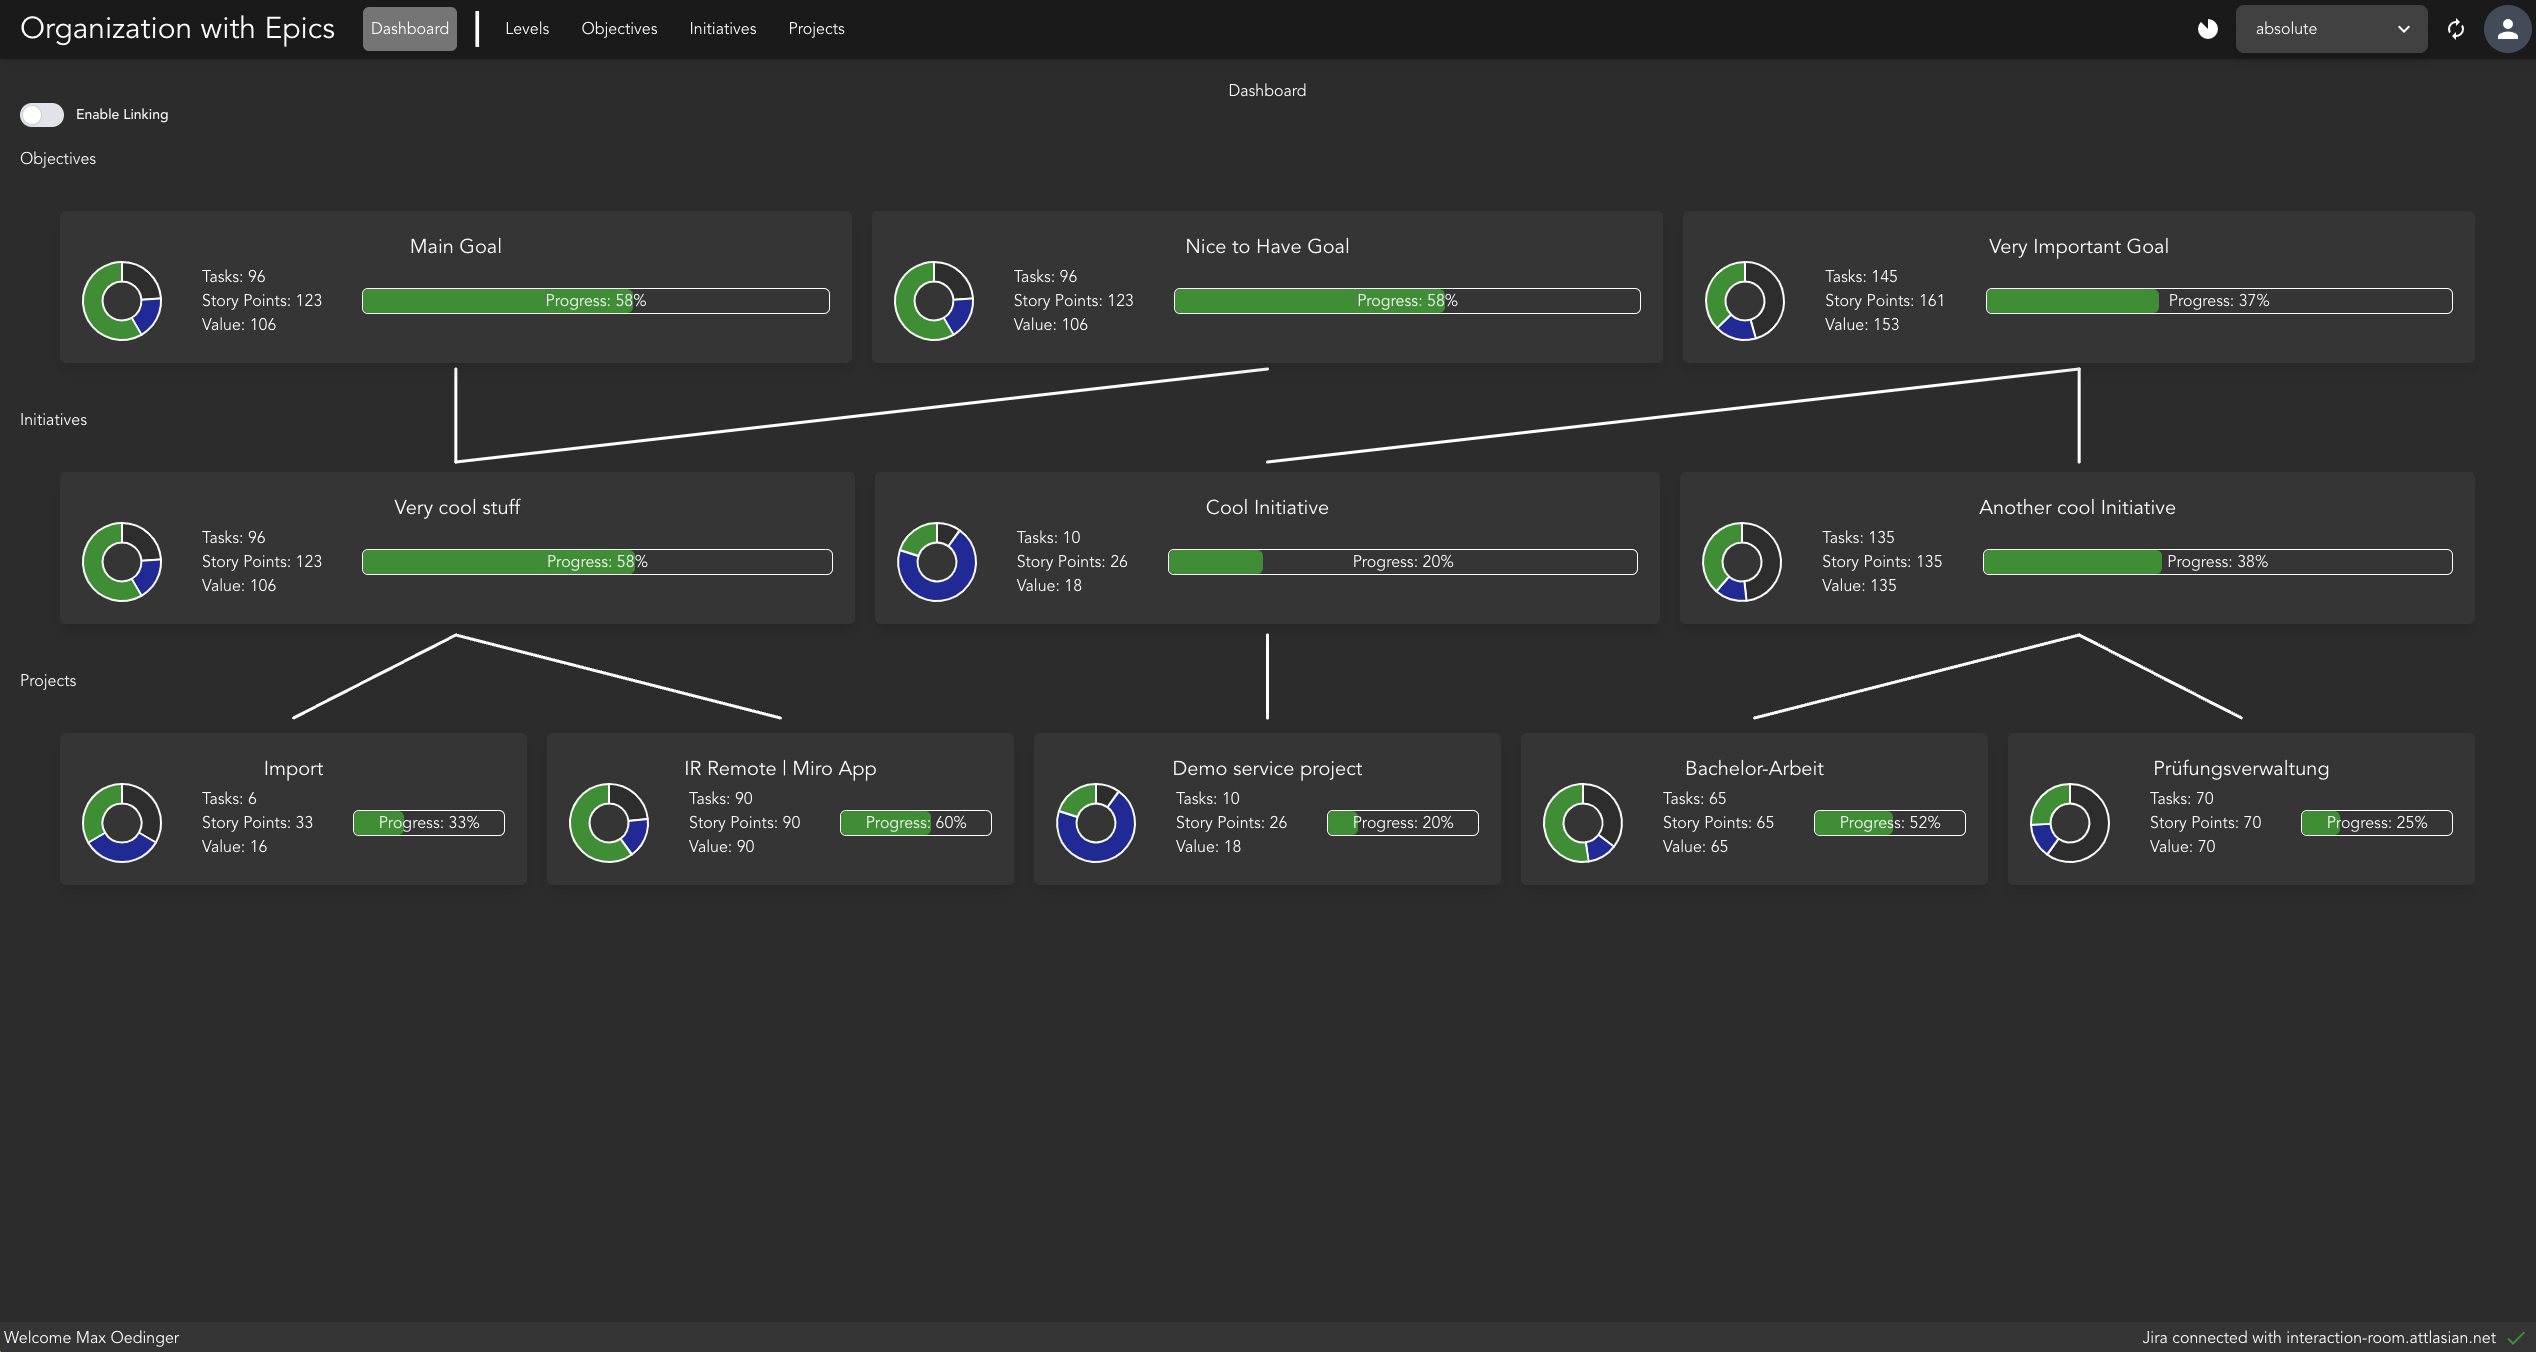
\includegraphics[width=\linewidth]{Dashboard_full}
        \captionof{figure}{Dashboard}
    \end{minipage}
\end{center}
\vspace{20pt}

Um die Verbindungslinien darzustellen wurde ein svg-Element im Hintergrund der Seite verwendet, welches die Verbindungslinien unabhängig von anderen Elementen auf der Seite darstellen kann. Die Start- und Endkoordinaten der Linien werden durch Positionen der Gruppen innerhalb der Seite berechnet. Dabei muss zusätzlich beachtet werden, wenn ein Level so viele Gruppen beinhaltet, dass sich einige Gruppen außerhalb des sichtbaren Bereichs befinden und durch einen Scroll in den sichtbaren bereich bewegt werden können. In diesem Fall müssen die Koordinaten der Linien entsprechend der Scroll-Position der verschobenen Gruppen neu berechnet werden.

\vspace{20pt}
\begin{center}
    \begin{minipage}{1\linewidth}
        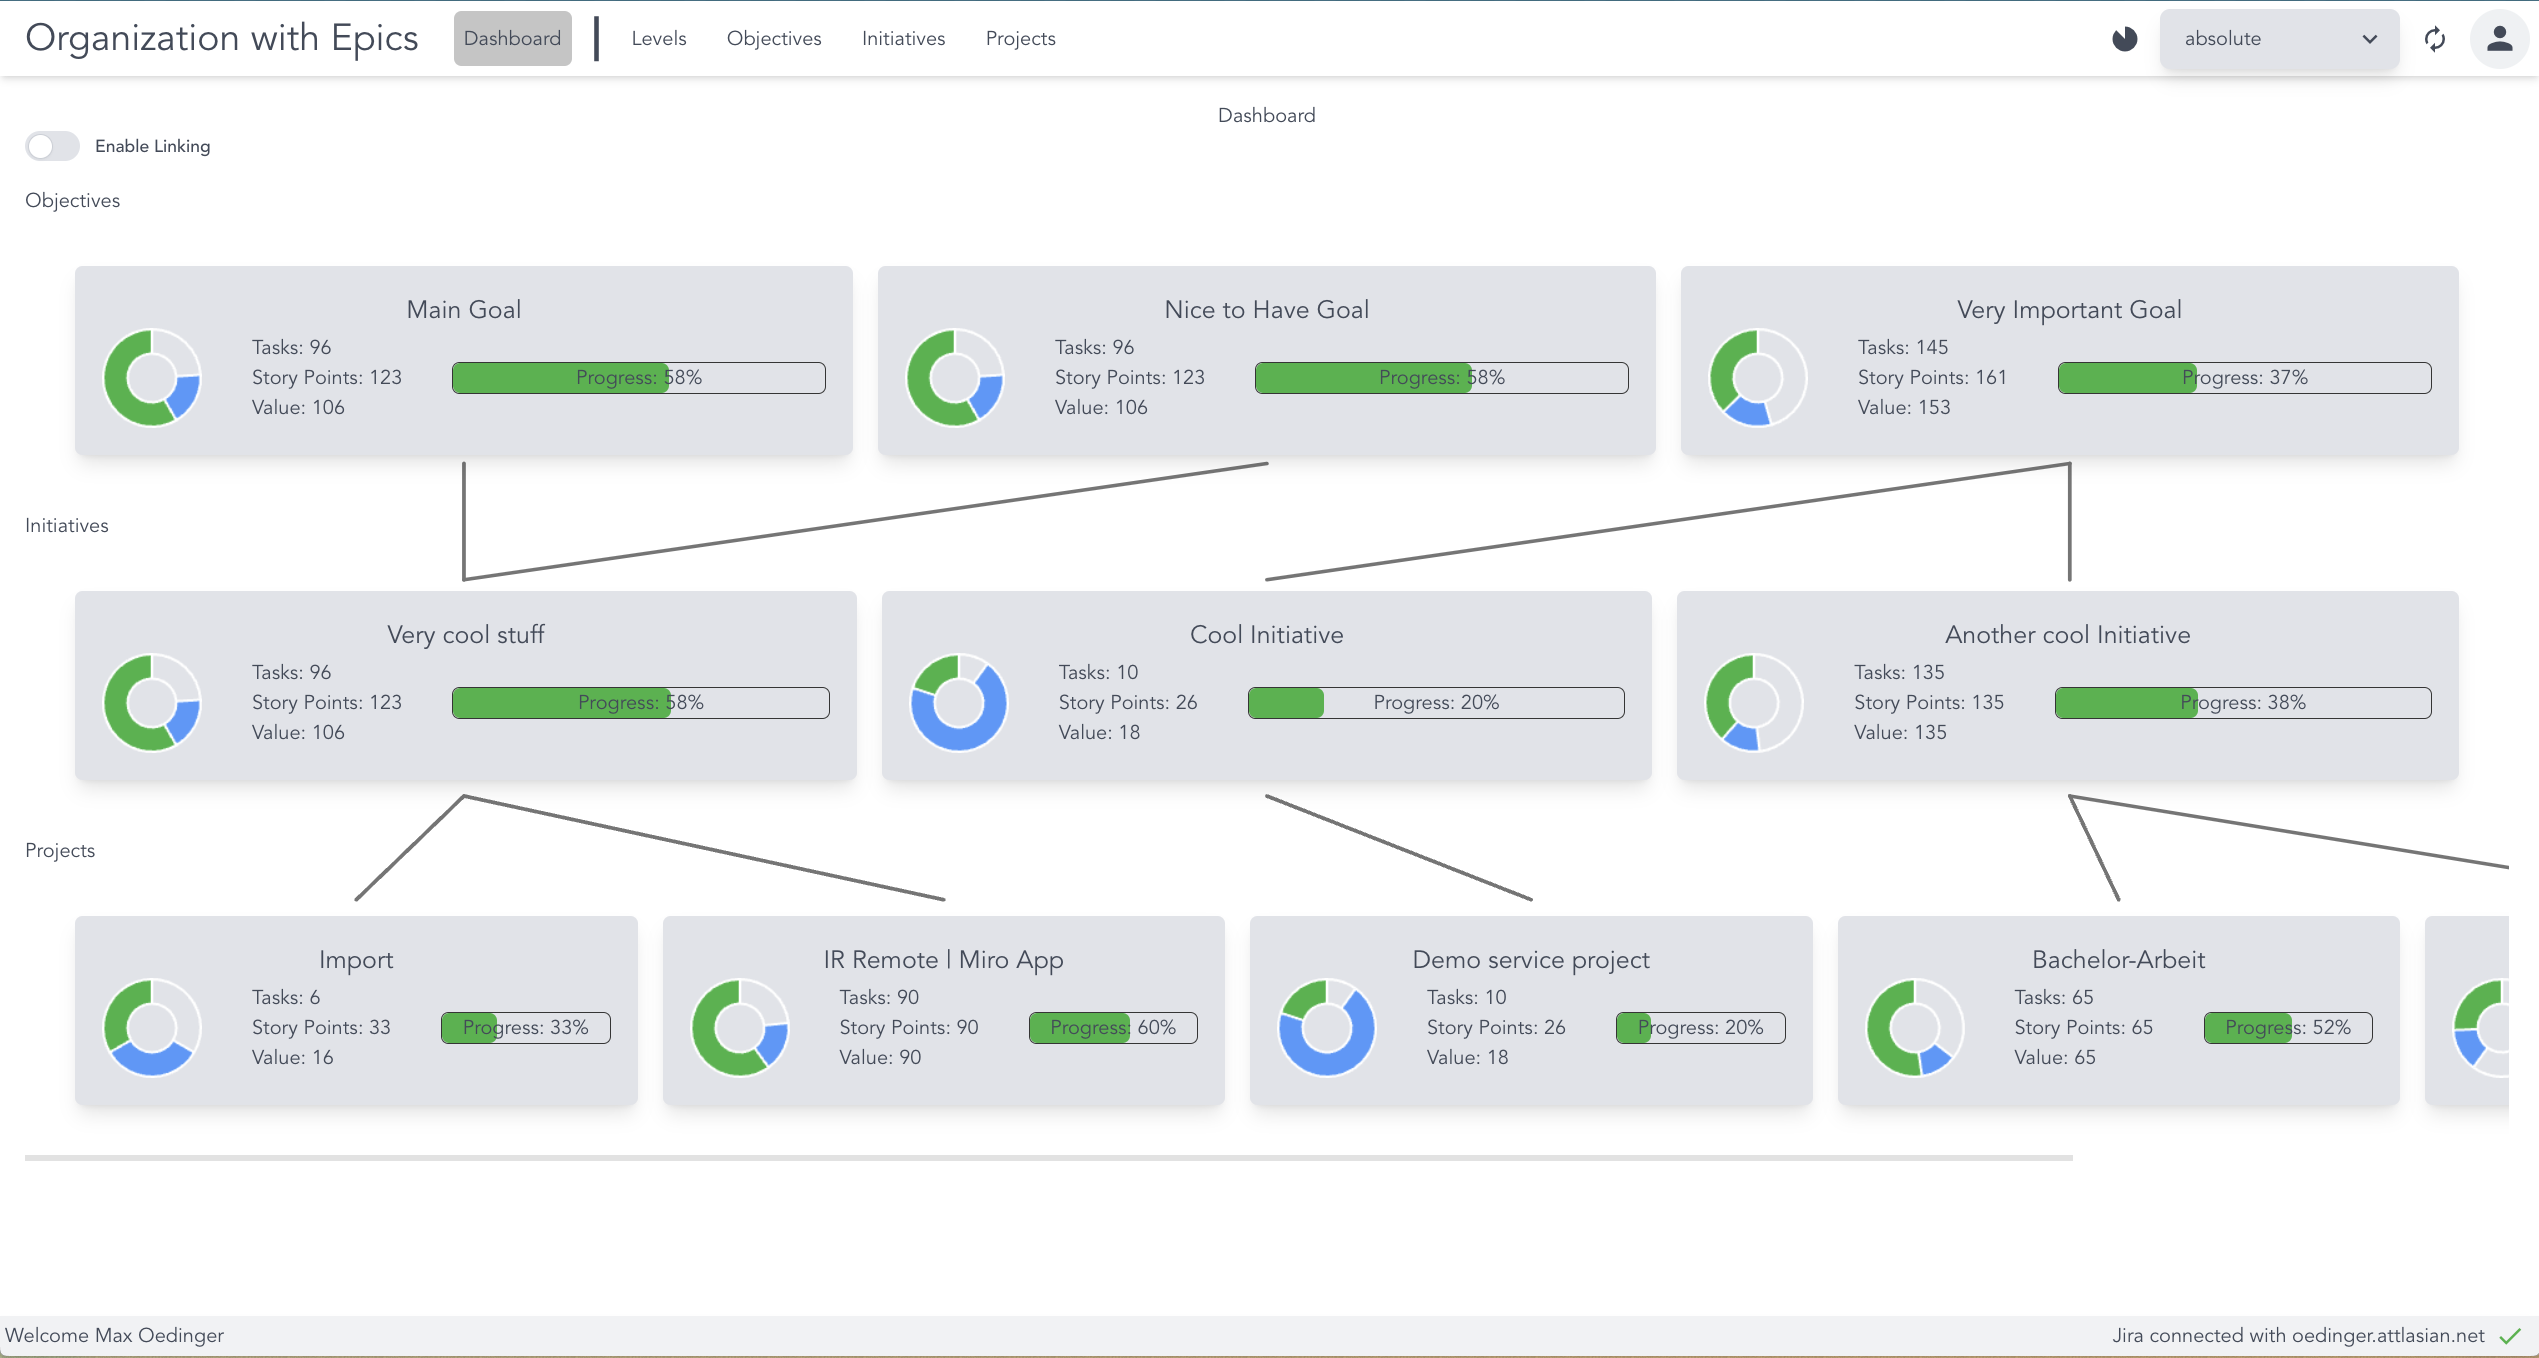
\includegraphics[width=\linewidth]{Dashboard_withScroll}
        \captionof{figure}{Dashboard mit scrollbaren Gruppen}
    \end{minipage}
\end{center}
\vspace{20pt}

Der Nutzer hat die Möglichkeit Verlinkung über ein Toggle zu aktivieren, wodurch über jeder Gruppe die verlinkt werden kann ein Punkt erscheint, den der Nutzer mit Drag and Drop verwenden kann um die Gruppe mit einer anderen Gruppe zu verbinden.
Anhand der Start-Position und aktuellen Position des Mauszeigers wird währenddessen eine neue Linies dargestellt, die dem Nutzer zeigt wie die Verbindung aussieht die er erzeugt. Anschließend werden die Verbindungsli
nien anhand der neuen Positionen der Gruppen erneut berechnet.

Zusätzlich zu den Linien kann der Nutzer den Mauszeiger über eine Gruppe bewegen, wodurch die Gruppe und die Gruppen die mit dieser Gruppe verknüpft sind, inklusieve aller relevanten Verbindungslinien blau hervorgehoben werden.

\vspace{20pt}
\begin{center}
    \begin{minipage}{1\linewidth}
        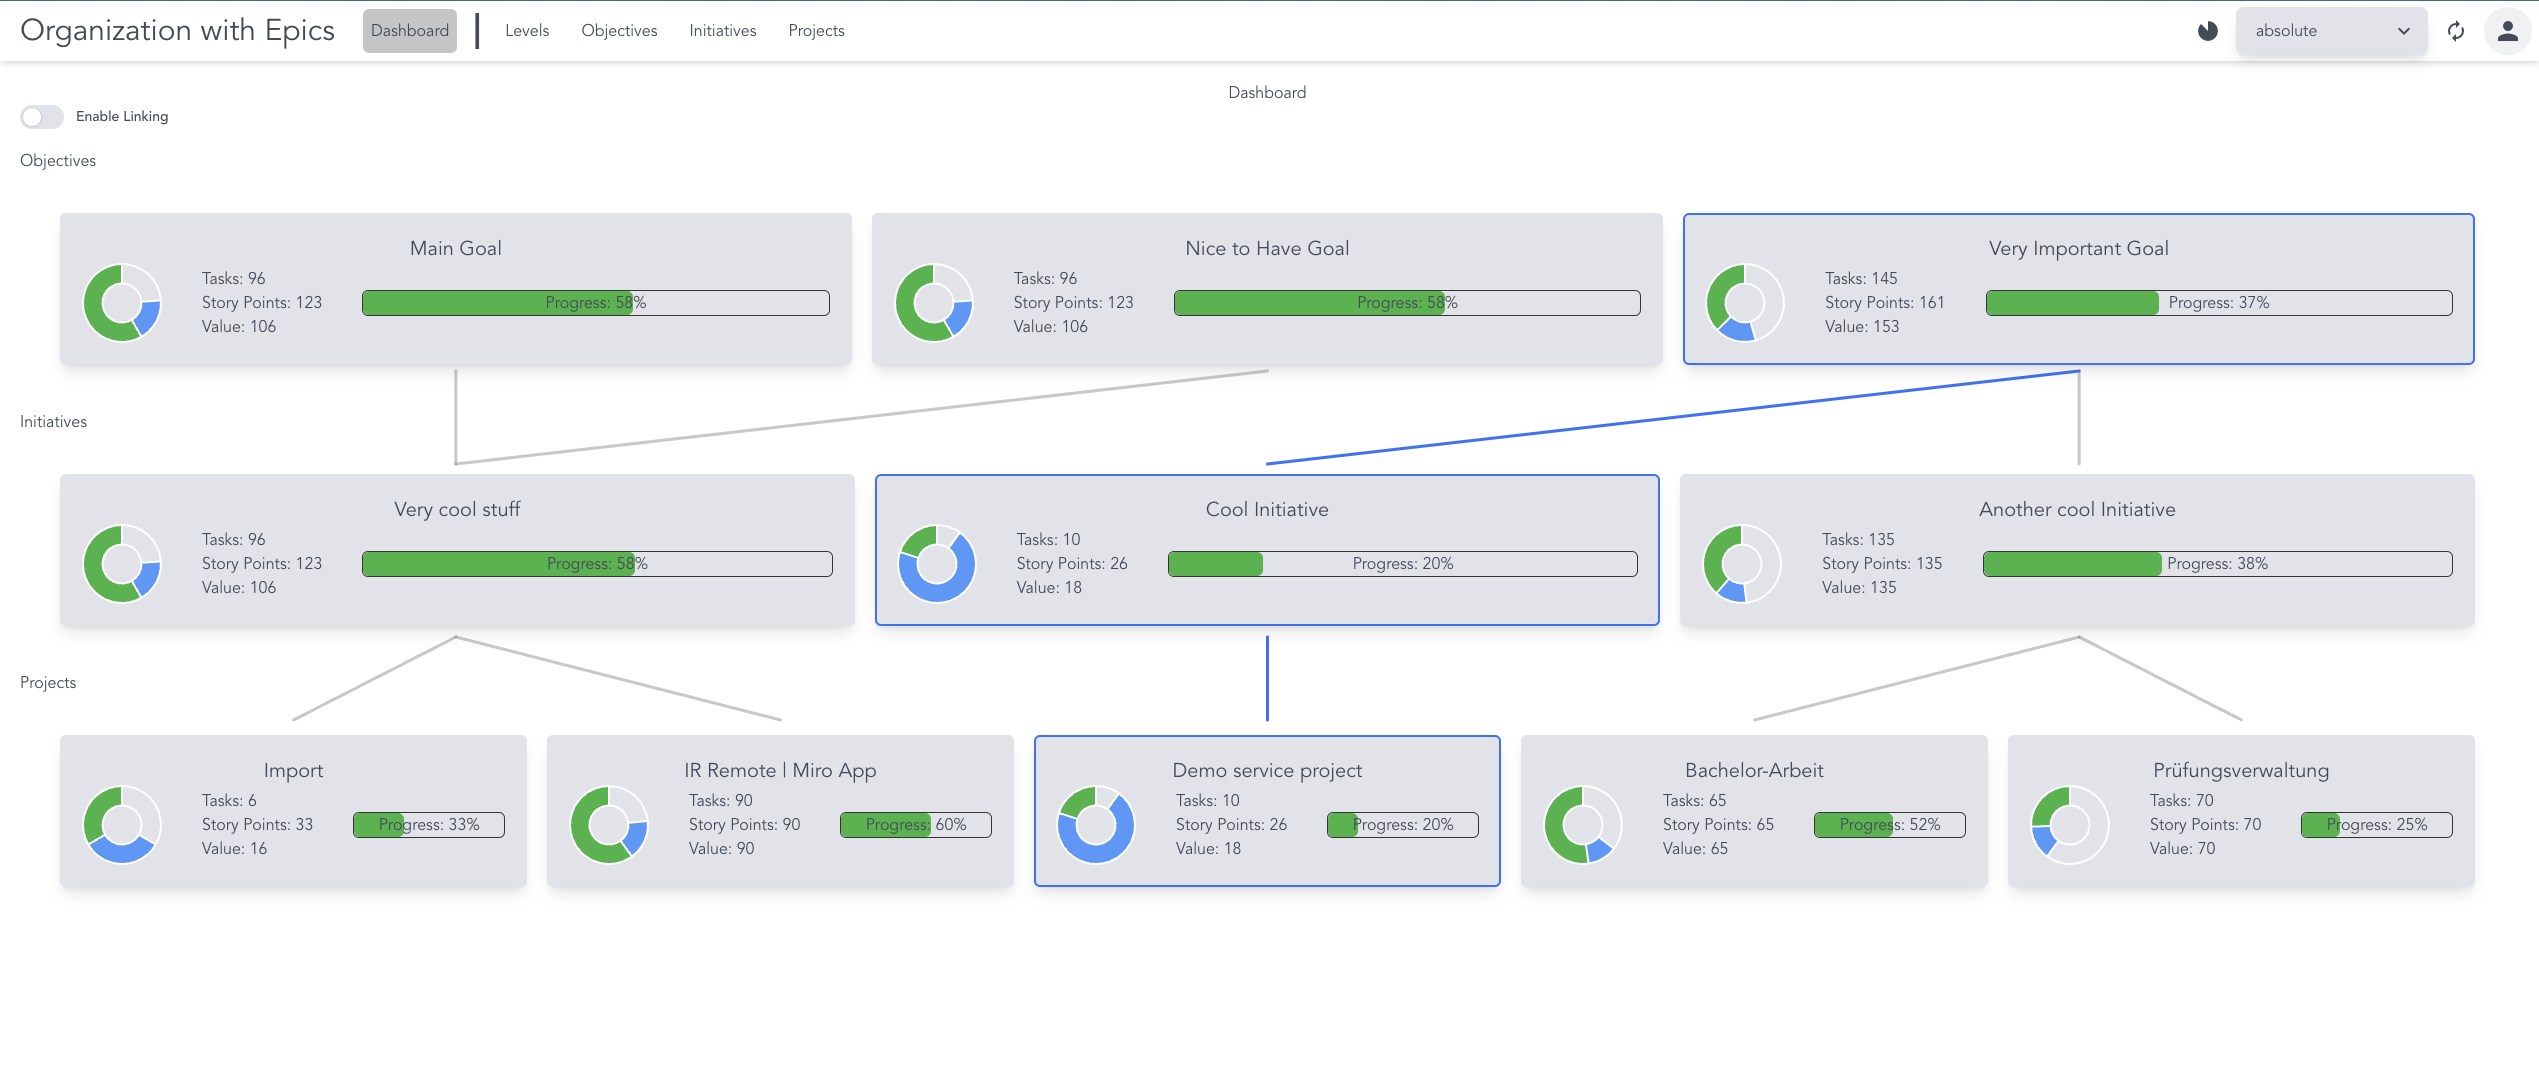
\includegraphics[width=\linewidth]{Dashboard_withHighlighting}
        \captionof{figure}{Dashboard mit hervorgehobenen Gruppen}
    \end{minipage}
\end{center}
\vspace{20pt}

\subsection{CI/CD}
Für eine schnelle und einfache Möglichkeit die Anwendung als produktive Anwendung zu testen und verbesserungen zu deployen wurde eine CI/CD-Pipeline mit GitHub-Actions eingerichtet. Die GitHub-Action definiert, wann die Pipeline ausgeführt werden soll und welche Schritte in der Pipeline ausgeführt werden sollen. Der Trigger für die Pipeline ist hier das Mergen und daraus resultierenden Schließen eines Pullrequests der als Ziel den main-Branch des Repositories hat.

\vspace{20pt}
\begin{center}
    \begin{minipage}{1\linewidth}
        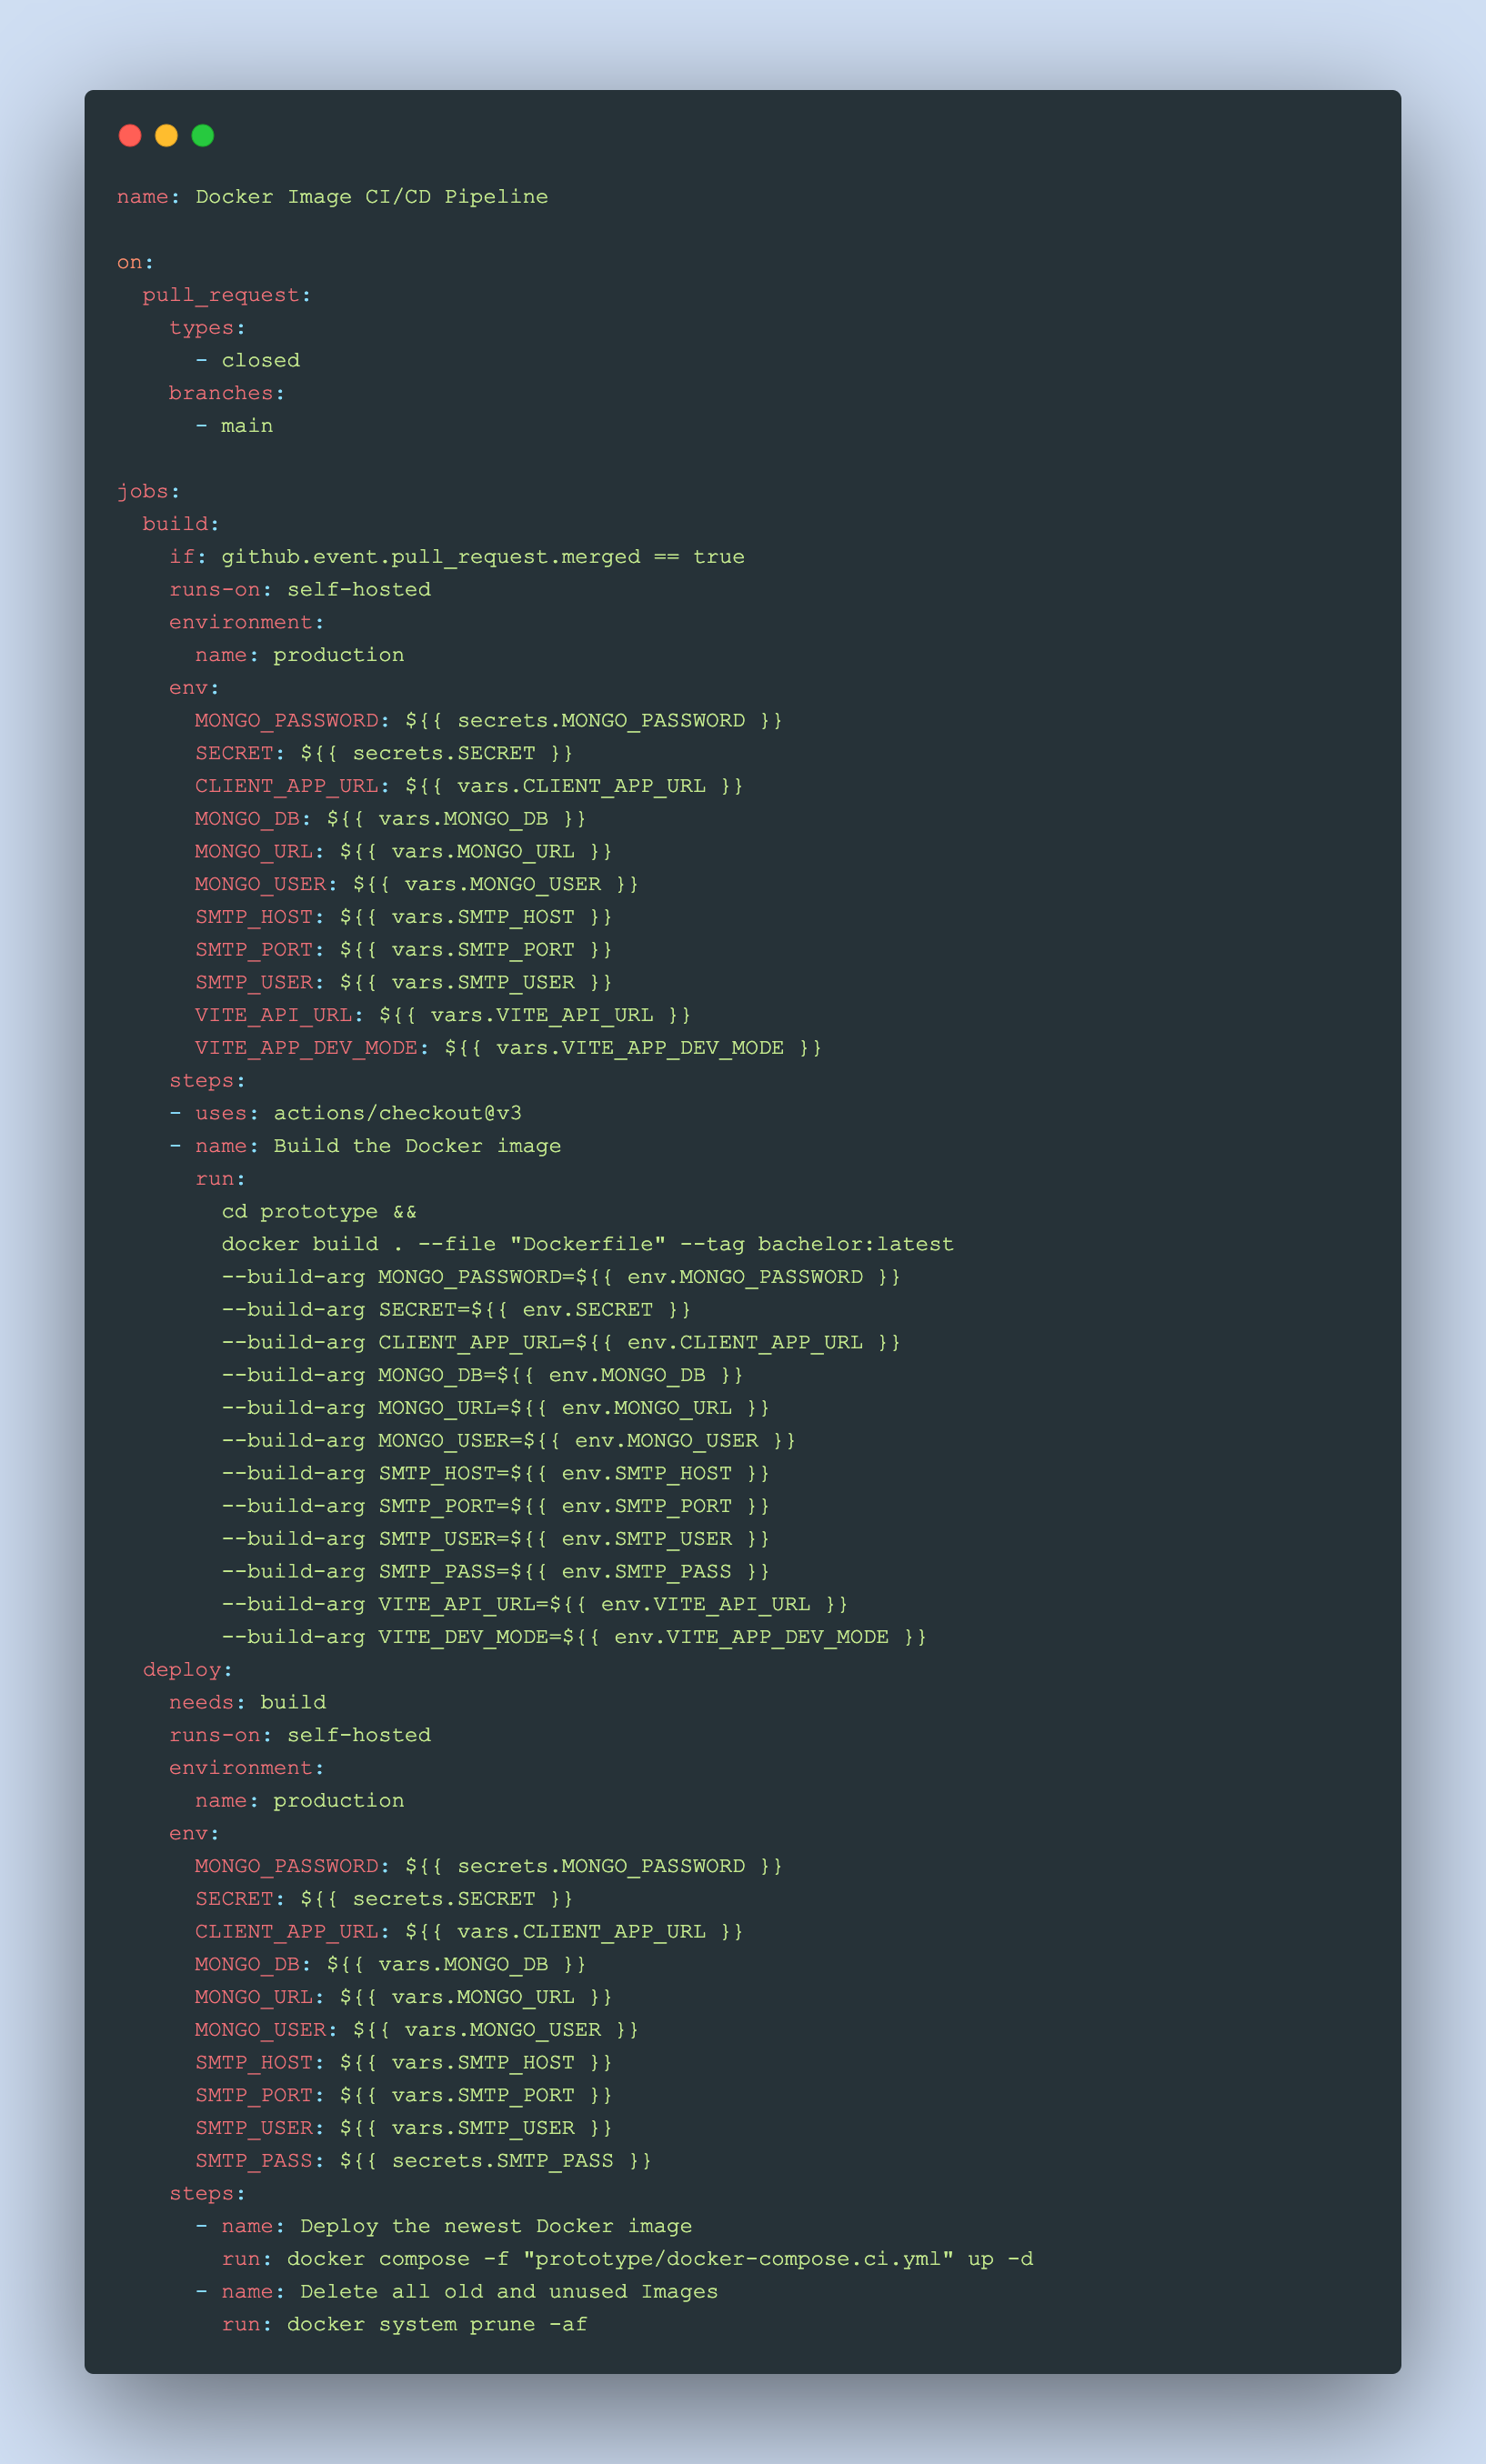
\includegraphics[width=\linewidth]{GitHubAction}
        \captionof{figure}{GitHub-Action}
    \end{minipage}
\end{center}
\vspace{20pt}

Die Pipeline besteht aus zwei Teilen, sogenannten Jobs: Build und Deploy.
Build erzeugt aus dem geupdateten Quellcode ein neues Docker-Image nach den konkreten Anweisungen die in dem Dockerfile im root-Verzeichnis des Prototypen definiert sind. Bei dem Dockerfile handlet es sich um ein multi-stage Dockerfile, welches in drei Schritten ein Image erzeugt. Diese drei Schritte sind:
frontend-build, backend-build, und production.

\vspace{20pt}
\begin{center}
    \begin{minipage}{1\linewidth}
        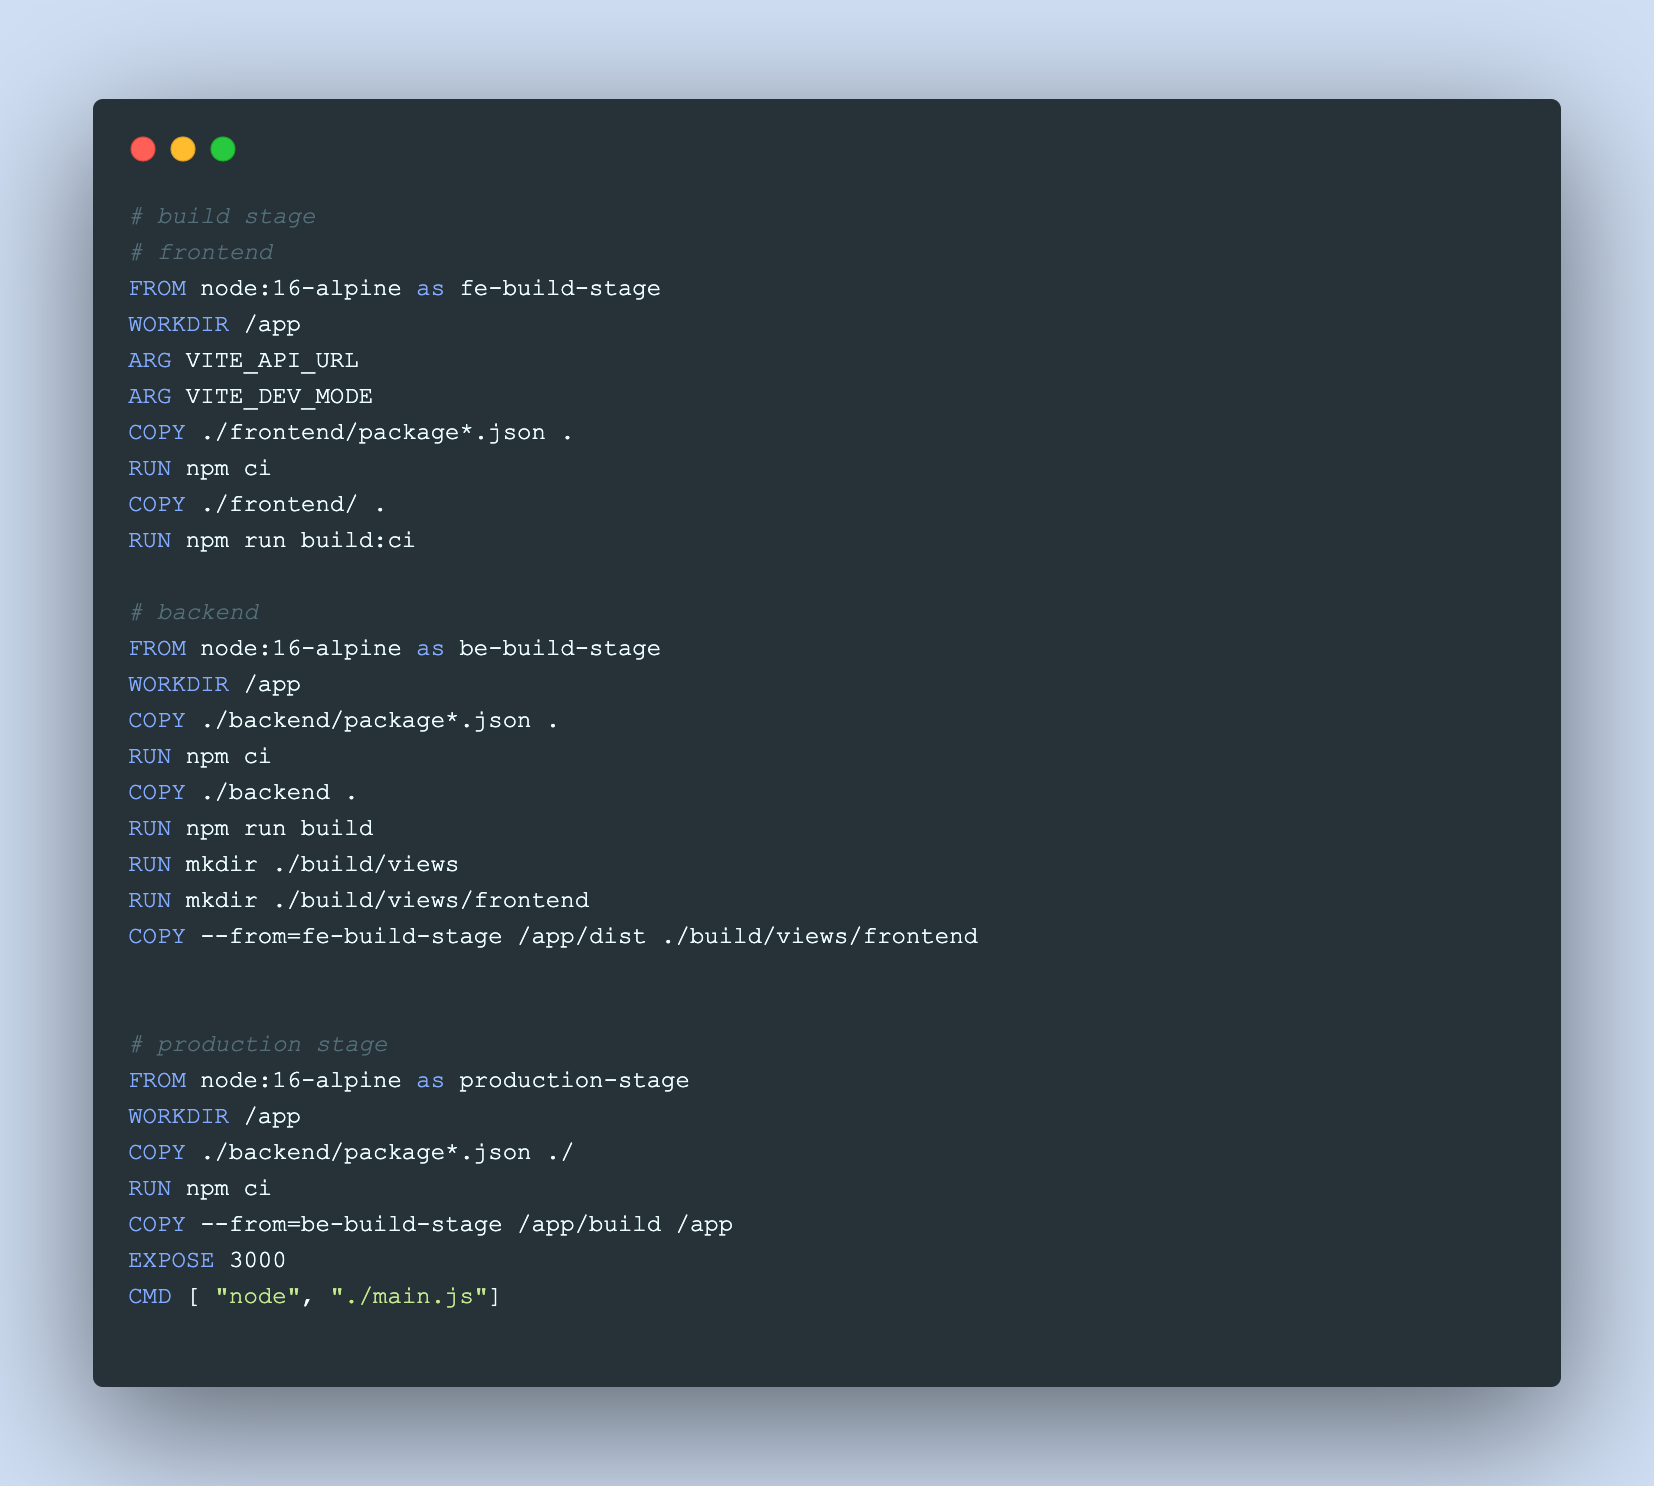
\includegraphics[width=\linewidth]{DockerFile}
        \captionof{figure}{Dockerfile zum Bauen des Images}
    \end{minipage}
\end{center}
\vspace{20pt}

Im ersten Schritt wird der Frontend-Code kompiliert. Im zweiten Schritt wird der Backend-Code kompiliert und das kompilierte Frontend aus dem ersten Schritt zur statischen auslieferung in einen bestimmten Ordner kopiert. Im dritten Schritt wird ein Node Image für die Produktivumgebung erzeugt welches das Kompilierte Backend inklusieve des Frontends enthält und mit einem Start-Befehl der Webserver gestartet wird.
Das resultierende Image, welches nun eine lauffähige Version der Anwendung enthält, wird anschließend als neueste Version des Images getagt.
Deploy führt ein Update der konkreten Produktivumgebung durch. Dazu wird das Image, welches im Build-Job erzeugt wurde, und das laufende Image ersetzt. Hierzu wird die Docker-Compose-Datei verwendet, welche die Konfiguration der Docker-Services der Produktivumgebung beschreibt. Diese Datei referenziert immer die neueste Version des gebauten Images und einen Reverse-Proxy-Service von "Traefik", welcher dazu dient das Portmapping auf dem Server zu übernehmen und ein SSL-Zertifikat für die angegebene Domain auszustellen.
Zuletzt werden alle alten und unbenutzt Images gelöscht.
\newpage
\section{Evaluation}
Im folgenden Kapitel wurde der Praxistest dokumentiert und die Ergebnisse ausgewertet, um eine Evaluation des prototypisch implementierten Konzepts durchzuführen und daraus entstandene Optimierungsvorschläge zu beschreiben.
\subsection{Praxistest}
Für den Praxistest wurden mit einem Experten, welcher Portfoliomanagement im täglichen Geschäft als Global Key Account Manager verwendet, praxisnahe Daten erstellt, die ein fiktives Unternehmen darstellen sollen. Anhand der Daten im Prototypen soll beurteilt werden, wie praxisrelevant die Funktionalitäten der Software sind und welche Verbesserungen und/oder Funktionalitäten für eine produktive Nutzung benötigt werden. Das Praxisprojekt beschreibt eine Unternehmensentwicklung für ein Unternehmen. Diese Unternehmensentwicklung stellt KPI's(Key Performance Indicators) als konkrete Unternehmensstrategie-Ziele dar, welche die oberste Ebene im Tool darstellt. Darunter unterteilt sich das Unternehmen in verschiedene Regionen, welche selbst eigene KPI's erfüllen sollen, die gemeinsam auf die KPI's in der obersten Ebene einzahlen. Diese Regionen unterteilen sich erneut in Subregions, welche wieder ihre eigenen KPI's erfüllen sollen. Unter diesen Subregions befindet sich eine HQ-Ebene, in der sich CoE's (Center of Excellence) befinden, welche dann mit den Projekten in der konkreten operativen Ebene darunter verknüpft sind.

\vspace{20pt}
\begin{center}
    \begin{minipage}{1\linewidth}
        \includegraphics[width=\linewidth]{Praxisdaten}
        \captionof{figure}{Dashboard mit Praxisdaten}
    \end{minipage}
\end{center}
\vspace{20pt}

\subsection{Optimierungsvorschläge}
Nach der Erstellung der Datenstruktur hat der Experte das Dashboard zu sehen bekommen und konnte sich in der Anwendung umsehen. Dabei wurden bewusste Entscheidungen, wie die fehlende Synchronisation und Autorisierung erläutert und begründet.
Das gegebene Feedback lässt sich in 3 Punkten zusammenfassen:

\begin{itemize}
    \item mehr Filterfunktionalitäten
    \item zeitbasierte Metriken
    \item möglichst vollständige Dokumentation für die dokumentierte Datenstruktur
\end{itemize}

Je größer und komplexer die Datenstruktur wurde, desto schwieriger wurde es die Übersicht über alle Elemente zu behalten. Da meist gar nicht alle Daten in jedem Kontext relevant sind, wäre eine Filterfunktionalität sinnvoll, insbesondere für Planungselemente, in denen noch kein Fortschritt sichtbar ist, da sie sich noch nicht in der Umsetzung befinden.

Fortschritt als aktuellen Wert sichtbar zu machen kann in vielen Situationen bereits bei der Entscheidungsfindung helfen, kann aber auch ohne Kontext von Fortschritt über Zeit irreführend sein. Zeitbasierte Metriken wie den Fortschritt über Zeit, Durchsatz oder die Velocity werden an dieser Stelle ebenfalls benötigt.

Die Datenstruktur sollte so vollständig wie möglich dokumentiert werden können, um effektiver Einigkeit über die Bedeutung der verschiedenen Ebenen und Elemente zu erzielen. Dokumentation sollte dabei direkt im Tool möglich sein.
\newpage
\section{Fazit}
In dieser Arbeit wurde ein Konzept für eine softwaregestützten Dokumentation von Unternehmensstrukturen für automatisierte Fortschrittsmessung und Werteorientierung entwickelt. Dazu wurde eine Datenstruktur entworfen, die die Abbildung von Unternehmensstrukturen, wie Sie für (agiles) Projekt-Portfoliomanagement verwendet werden und eine Datenaggregation für den Fortschritt ermöglicht. Sie soll dabei möglichst flexibel sein, um unabhängig von der konkreten Unternehmensstruktur bzw. dem verwendeten Management-Framework verwendet werden zu können. Die Datenstruktur wurde in einem Prototyp implementiert, der die Funktionalitäten der Datenstruktur in einer Webanwendung umsetzt, um damit das Konzept in einem Praxistest zu evaluieren. Dazu wurde eine fiktive praxisnahe Unternehmensstruktur mit der Unterstützung eines Experten in der Anwendung abgebildet. Dieses Beispiel wurde dann verwendet, um die Anwendung selbst zu testen.

\subsection{Ergebnis}
Die Ergebnisse des Literatur-Reviews zeigten, dass Unternehmen Entscheidungen durch softwaregestützte Dokumentation und automatisiertes Reporting unterstützen sollten, um Entscheidungsfindung zu systematisieren und Entscheidungsqualität zu steigern. Die Ergebnisse des Praxistests zeigten, dass die Datenstruktur dazu in der Lage ist Unternehmensstrukturen abzubilden und die Fortschrittsaggregation eine Form von automatisiertem Reporting darstellt. Des Weiteren sind zwei Kernfunktionalitäten während der Entwicklung des Konzepts identifiziert worden, welche aufgrund der Komplexität nicht implementiert wurden: Die Synchronisation mit operativen Tools wie Jira, anstelle eines einfachen Imports und die Autorisierung und Verwaltung verschiedener Nutzer für Lesebeschränkungen. Außerdem wurden durch den Praxistest drei weitere Funktionalitäten identifiziert, mit denen die Anwendung möglicherweise produktive Anwendung finden kann.

\subsection{Reflexion}
Das Konzept kann Unternehmensstrukturen als solches dokumentieren, sollte aber weitere Möglichkeiten bieten den Kontext von z. B. verschiedenen Ebenen besser zu beschreiben. Die Fortschrittsaggregation ist eine Möglichkeit für eine Unterstützung von wertebasierter Entscheidungsfindung, reicht aber alleine nicht aus, um effektive die Entscheidungen zu verbessern. Hierzu werden vor allem zeitbasierte Metriken benötigt. Die beiden zuvor erwähnten Funktionalitäten, welche bewusst nicht implementiert wurden, werden definitiv benötigt, um die Anwendung produktiv und Unternehmensweit zu verwenden. Die Visualisierung der Datenstruktur kann ebenfalls verbessert werden, indem Filterfunktionalitäten implementieren, welche die Übersicht über größere Strukturen gewährleisten können und den Fokus auf die relevanten Informationen legen.

Für die Berechnung von zeitbasierten Metriken wird in der Datenstruktur eine zeitliche Dimension benötigt, mit der Änderungen über Zeit gespeichert werden können.

Die Datenaggregation findet zurzeit im Frontend, also dem Nutzer-seitigen Teil der Anwendung, statt. Dies könnte insbesondere bei komplexeren Metriken sinnvoller im Server-seitigen Teil der Anwendung stattfinden. Auch die Kalkulation der Metriken wie Valocity o. Ä. könnte vor allem für zukünftig Synchronisierte Projekt aus anderen Tools, wie z. B. Jira bezogen werden, die ohnehin solche Reports zur Verfügung stellen.

\subsection{Ausblick}
Sowohl das entwickelte Konzept, als auch die Implementierung dessen, erlauben ohne weitere Komplikation eine Umsetzung aller identifizierten fehlenden Funktionalitäten und Verbessungen. Hierbei sollten weitere Metriken, die über die Fortschrittsmessung hinaus gehen, implementiert werden, da es sich bei dieser Arbeit nur um einen Prototypen handelt, der die Aggregation von Daten über mehrere Ebenen hinweg am Beispiel der Fortschrittsmessung demonstriert.
Mit dieser Umsetzung kann das Konzept dann auch realistisch in einem tatsächlichen Praxisumfeld über einen längeren Zeitraum getestet werden, um die Effektivität der Unterstützung von wertebasierter Entscheidungsfindung zu evaluieren.


\newpage
\addcontentsline{toc}{section}{Literaturverzeichnis}
\printbibliography

\newpage
\appendix
\section{Anhang}
\subsection{Anhang 1}
\newpage
\addcontentsline{toc}{section}{Selbständigkeitserklärung}
\section*{Selbständigkeitserklärung}
Hiermit erkläre ich, Maximilian Oedinger, dass ich die hier vorliegende Arbeit selbst-ständig und ohne unerlaubte Hilfsmittel angefertigt habe. Informationen, die
anderen Werken oder Quellen dem Wortlaut oder dem Sinn nach entnommen sind, habe ich kenntlich gemacht und mit exakter Quellenangabe
versehen. Sätze oder Satzteile, die wörtlich übernommen wurden, wurden
als Zitate gekennzeichnet. Die hier vorliegende Arbeit wurde noch an
keiner anderen Stelle zur Prüfung vorgelegt und weder ganz noch in
Auszügen veröffentlicht. Bis zur Veröffentlichung der Ergebnisse durch den
Prüfungsausschuss werde ich eine Kopie dieser Studienarbeit aufbewahren und wenn nötig zugänglich machen.

\end{document}
